\documentclass[twoside]{book}

% Packages required by doxygen
\usepackage{fixltx2e}
\usepackage{calc}
\usepackage{doxygen}
\usepackage[export]{adjustbox} % also loads graphicx
\usepackage{graphicx}
\usepackage[utf8]{inputenc}
\usepackage{makeidx}
\usepackage{multicol}
\usepackage{multirow}
\PassOptionsToPackage{warn}{textcomp}
\usepackage{textcomp}
\usepackage[nointegrals]{wasysym}
\usepackage[table]{xcolor}

% Font selection
\usepackage[T1]{fontenc}
\usepackage[scaled=.90]{helvet}
\usepackage{courier}
\usepackage{amssymb}
\usepackage{sectsty}
\renewcommand{\familydefault}{\sfdefault}
\allsectionsfont{%
  \fontseries{bc}\selectfont%
  \color{darkgray}%
}
\renewcommand{\DoxyLabelFont}{%
  \fontseries{bc}\selectfont%
  \color{darkgray}%
}
\newcommand{\+}{\discretionary{\mbox{\scriptsize$\hookleftarrow$}}{}{}}

% Page & text layout
\usepackage{geometry}
\geometry{%
  a4paper,%
  top=2.5cm,%
  bottom=2.5cm,%
  left=2.5cm,%
  right=2.5cm%
}
\tolerance=750
\hfuzz=15pt
\hbadness=750
\setlength{\emergencystretch}{15pt}
\setlength{\parindent}{0cm}
\setlength{\parskip}{3ex plus 2ex minus 2ex}
\makeatletter
\renewcommand{\paragraph}{%
  \@startsection{paragraph}{4}{0ex}{-1.0ex}{1.0ex}{%
    \normalfont\normalsize\bfseries\SS@parafont%
  }%
}
\renewcommand{\subparagraph}{%
  \@startsection{subparagraph}{5}{0ex}{-1.0ex}{1.0ex}{%
    \normalfont\normalsize\bfseries\SS@subparafont%
  }%
}
\makeatother

% Headers & footers
\usepackage{fancyhdr}
\pagestyle{fancyplain}
\fancyhead[LE]{\fancyplain{}{\bfseries\thepage}}
\fancyhead[CE]{\fancyplain{}{}}
\fancyhead[RE]{\fancyplain{}{\bfseries\leftmark}}
\fancyhead[LO]{\fancyplain{}{\bfseries\rightmark}}
\fancyhead[CO]{\fancyplain{}{}}
\fancyhead[RO]{\fancyplain{}{\bfseries\thepage}}
\fancyfoot[LE]{\fancyplain{}{}}
\fancyfoot[CE]{\fancyplain{}{}}
\fancyfoot[RE]{\fancyplain{}{\bfseries\scriptsize Generated by Doxygen }}
\fancyfoot[LO]{\fancyplain{}{\bfseries\scriptsize Generated by Doxygen }}
\fancyfoot[CO]{\fancyplain{}{}}
\fancyfoot[RO]{\fancyplain{}{}}
\renewcommand{\footrulewidth}{0.4pt}
\renewcommand{\chaptermark}[1]{%
  \markboth{#1}{}%
}
\renewcommand{\sectionmark}[1]{%
  \markright{\thesection\ #1}%
}

% Indices & bibliography
\usepackage{natbib}
\usepackage[titles]{tocloft}
\setcounter{tocdepth}{3}
\setcounter{secnumdepth}{5}
\makeindex

% Hyperlinks (required, but should be loaded last)
\usepackage{ifpdf}
\ifpdf
  \usepackage[pdftex,pagebackref=true]{hyperref}
\else
  \usepackage[ps2pdf,pagebackref=true]{hyperref}
\fi
\hypersetup{%
  colorlinks=true,%
  linkcolor=blue,%
  citecolor=blue,%
  unicode%
}

% Custom commands
\newcommand{\clearemptydoublepage}{%
  \newpage{\pagestyle{empty}\cleardoublepage}%
}

\usepackage{caption}
\captionsetup{labelsep=space,justification=centering,font={bf},singlelinecheck=off,skip=4pt,position=top}

%===== C O N T E N T S =====

\begin{document}

% Titlepage & ToC
\hypersetup{pageanchor=false,
             bookmarksnumbered=true,
             pdfencoding=unicode
            }
\pagenumbering{alph}
\begin{titlepage}
\vspace*{7cm}
\begin{center}%
{\Large F\+AM Osprey \\[1ex]\large v0.\+9 }\\
\vspace*{1cm}
{\large Generated by Doxygen 1.8.13}\\
\end{center}
\end{titlepage}
\clearemptydoublepage
\pagenumbering{roman}
\tableofcontents
\clearemptydoublepage
\pagenumbering{arabic}
\hypersetup{pageanchor=true}

%--- Begin generated contents ---
\chapter{Class Index}
\section{Class List}
Here are the classes, structs, unions and interfaces with brief descriptions\+:\begin{DoxyCompactList}
\item\contentsline{section}{\hyperlink{class_c_h_i___o_s_p_r_e_y}{C\+H\+I\+\_\+\+O\+S\+P\+R\+EY} }{\pageref{class_c_h_i___o_s_p_r_e_y}}{}
\item\contentsline{section}{\hyperlink{class_c_h_i___v_e_c_t_o_r}{C\+H\+I\+\_\+\+V\+E\+C\+T\+O\+R$<$ Vector\+Type $>$} }{\pageref{class_c_h_i___v_e_c_t_o_r}}{}
\end{DoxyCompactList}

\chapter{File Index}
\section{File List}
Here is a list of all documented files with brief descriptions\+:\begin{DoxyCompactList}
\item\contentsline{section}{Project1/\hyperlink{main_8cpp}{main.\+cpp} }{\pageref{main_8cpp}}{}
\item\contentsline{section}{Project1/\+C\+H\+I\+\_\+\+O\+S\+P\+R\+E\+Y/\hyperlink{chi__osprey_8h}{chi\+\_\+osprey.\+h} }{\pageref{chi__osprey_8h}}{}
\item\contentsline{section}{Project1/\+C\+H\+I\+\_\+\+O\+S\+P\+R\+E\+Y/\hyperlink{chi__osprey__00__constrdestr_8cpp}{chi\+\_\+osprey\+\_\+00\+\_\+constrdestr.\+cpp} }{\pageref{chi__osprey__00__constrdestr_8cpp}}{}
\item\contentsline{section}{Project1/\+C\+H\+I\+\_\+\+O\+S\+P\+R\+E\+Y/\hyperlink{chi__osprey__01__functions_8cpp}{chi\+\_\+osprey\+\_\+01\+\_\+functions.\+cpp} }{\pageref{chi__osprey__01__functions_8cpp}}{}
\item\contentsline{section}{Project1/\+C\+H\+I\+\_\+\+V\+E\+C\+T\+O\+R/\hyperlink{chi__vector_8h}{chi\+\_\+vector.\+h} }{\pageref{chi__vector_8h}}{}
\end{DoxyCompactList}

\chapter{Class Documentation}
\hypertarget{class_c_h_i___o_s_p_r_e_y}{}\section{C\+H\+I\+\_\+\+O\+S\+P\+R\+EY Class Reference}
\label{class_c_h_i___o_s_p_r_e_y}\index{C\+H\+I\+\_\+\+O\+S\+P\+R\+EY@{C\+H\+I\+\_\+\+O\+S\+P\+R\+EY}}


{\ttfamily \#include $<$chi\+\_\+osprey.\+h$>$}



Collaboration diagram for C\+H\+I\+\_\+\+O\+S\+P\+R\+EY\+:\nopagebreak
\begin{figure}[H]
\begin{center}
\leavevmode
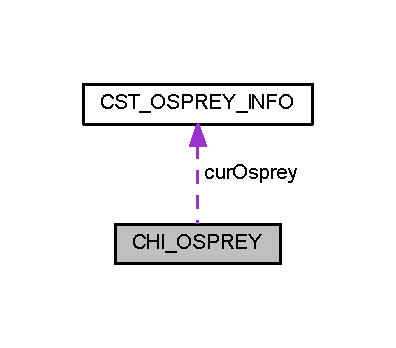
\includegraphics[width=190pt]{db/d2b/class_c_h_i___o_s_p_r_e_y__coll__graph}
\end{center}
\end{figure}
\subsection*{Public Member Functions}
\begin{DoxyCompactItemize}
\item 
\hyperlink{class_c_h_i___o_s_p_r_e_y_ab53100273a3288187b5f49ee4d14f1b2_ab53100273a3288187b5f49ee4d14f1b2}{C\+H\+I\+\_\+\+O\+S\+P\+R\+EY} ()
\item 
\hyperlink{class_c_h_i___o_s_p_r_e_y_adfb630759c9dfe8d0d55079cf1e2bf4e_adfb630759c9dfe8d0d55079cf1e2bf4e}{$\sim$\+C\+H\+I\+\_\+\+O\+S\+P\+R\+EY} ()
\item 
\mbox{\Hypertarget{class_c_h_i___o_s_p_r_e_y_ac8624fc743990f8b4777f424e3d36bc3}\label{class_c_h_i___o_s_p_r_e_y_ac8624fc743990f8b4777f424e3d36bc3}} 
void {\bfseries Osprey\+Initialize} (int osp\+ID, bool user\+Mode)
\item 
\mbox{\Hypertarget{class_c_h_i___o_s_p_r_e_y_adad798cc07dd2c23f939891eceb83a99}\label{class_c_h_i___o_s_p_r_e_y_adad798cc07dd2c23f939891eceb83a99}} 
void {\bfseries Osprey\+Pull\+Spectrums} (int osp\+ID, int sleep\+Time)
\end{DoxyCompactItemize}
\subsection*{Public Attributes}
\begin{DoxyCompactItemize}
\item 
\mbox{\Hypertarget{class_c_h_i___o_s_p_r_e_y_a54c8ff029f901c396da3c0456da1bd12}\label{class_c_h_i___o_s_p_r_e_y_a54c8ff029f901c396da3c0456da1bd12}} 
Dev\+Cntl\+::\+I\+Device\+Ptr {\bfseries dtb}
\item 
\mbox{\Hypertarget{class_c_h_i___o_s_p_r_e_y_aea5477286efa68b5b232371a4a031054}\label{class_c_h_i___o_s_p_r_e_y_aea5477286efa68b5b232371a4a031054}} 
int {\bfseries spectrum\+Values} \mbox{[}2048\mbox{]}
\item 
\mbox{\Hypertarget{class_c_h_i___o_s_p_r_e_y_ab55bdfc12320647a3454d777f61769fe}\label{class_c_h_i___o_s_p_r_e_y_ab55bdfc12320647a3454d777f61769fe}} 
long {\bfseries osp\+Input}
\item 
\mbox{\Hypertarget{class_c_h_i___o_s_p_r_e_y_a15536653f0d0c95d45f82b5e8f3938d4}\label{class_c_h_i___o_s_p_r_e_y_a15536653f0d0c95d45f82b5e8f3938d4}} 
variant\+\_\+t {\bfseries mem\+Group}
\item 
\mbox{\Hypertarget{class_c_h_i___o_s_p_r_e_y_aa268b72d81e7fd8a21478875e40d69d6}\label{class_c_h_i___o_s_p_r_e_y_aa268b72d81e7fd8a21478875e40d69d6}} 
variant\+\_\+t {\bfseries spectrum\+Mode}
\item 
\mbox{\Hypertarget{class_c_h_i___o_s_p_r_e_y_ace6e738bee717acedb8402b0ebceb5a7}\label{class_c_h_i___o_s_p_r_e_y_ace6e738bee717acedb8402b0ebceb5a7}} 
variant\+\_\+t {\bfseries preset\+Mode}
\item 
\mbox{\Hypertarget{class_c_h_i___o_s_p_r_e_y_a67d74f515fd3bd7c72918a8069a32871}\label{class_c_h_i___o_s_p_r_e_y_a67d74f515fd3bd7c72918a8069a32871}} 
variant\+\_\+t {\bfseries voltage\+Status}
\item 
\mbox{\Hypertarget{class_c_h_i___o_s_p_r_e_y_a46a460dfc280246a2f05cc3e6ba16b36}\label{class_c_h_i___o_s_p_r_e_y_a46a460dfc280246a2f05cc3e6ba16b36}} 
V\+A\+R\+I\+A\+NT {\bfseries args}
\item 
\mbox{\Hypertarget{class_c_h_i___o_s_p_r_e_y_a41b322381bcb58713cdd103862054607}\label{class_c_h_i___o_s_p_r_e_y_a41b322381bcb58713cdd103862054607}} 
std\+::string {\bfseries user}
\item 
\mbox{\Hypertarget{class_c_h_i___o_s_p_r_e_y_a5d766efe3728f2509929ff32511cfc52}\label{class_c_h_i___o_s_p_r_e_y_a5d766efe3728f2509929ff32511cfc52}} 
std\+::string {\bfseries password}
\item 
\mbox{\Hypertarget{class_c_h_i___o_s_p_r_e_y_aef7179a7b0f4c1f6d07d3a81c18df14f}\label{class_c_h_i___o_s_p_r_e_y_aef7179a7b0f4c1f6d07d3a81c18df14f}} 
std\+::string {\bfseries ip\+Address}
\item 
\mbox{\Hypertarget{class_c_h_i___o_s_p_r_e_y_a1aadac7d3240a6d8dfaef39f00a8807b}\label{class_c_h_i___o_s_p_r_e_y_a1aadac7d3240a6d8dfaef39f00a8807b}} 
\hyperlink{chi__osprey_8h_d2/d7a/struct_c_s_t___o_s_p_r_e_y___i_n_f_o}{C\+S\+T\+\_\+\+O\+S\+P\+R\+E\+Y\+\_\+\+I\+N\+FO} $\ast$ {\bfseries cur\+Osprey}
\item 
\mbox{\Hypertarget{class_c_h_i___o_s_p_r_e_y_a7551a497cca8e0aaf4c7e192fb9a7e50}\label{class_c_h_i___o_s_p_r_e_y_a7551a497cca8e0aaf4c7e192fb9a7e50}} 
int {\bfseries channel} \mbox{[}6\mbox{]}
\item 
\mbox{\Hypertarget{class_c_h_i___o_s_p_r_e_y_a4671cf64201d511463c11e1f285a8d36}\label{class_c_h_i___o_s_p_r_e_y_a4671cf64201d511463c11e1f285a8d36}} 
int {\bfseries lower\+Bound} \mbox{[}6\mbox{]}
\item 
\mbox{\Hypertarget{class_c_h_i___o_s_p_r_e_y_ae9b94c01ae05d3a4152cf023b30cc3e5}\label{class_c_h_i___o_s_p_r_e_y_ae9b94c01ae05d3a4152cf023b30cc3e5}} 
int {\bfseries upper\+Bound} \mbox{[}6\mbox{]}
\item 
\mbox{\Hypertarget{class_c_h_i___o_s_p_r_e_y_a20d5a98d264b3c6390b5c74732aee879}\label{class_c_h_i___o_s_p_r_e_y_a20d5a98d264b3c6390b5c74732aee879}} 
bool {\bfseries user\+Mode}
\item 
\mbox{\Hypertarget{class_c_h_i___o_s_p_r_e_y_a70b0ff2a6aef4ed86c32f6841e28da86}\label{class_c_h_i___o_s_p_r_e_y_a70b0ff2a6aef4ed86c32f6841e28da86}} 
bool {\bfseries first\+Cycle}
\end{DoxyCompactItemize}


\subsection{Detailed Description}
Object for handling Osprey. \begin{DoxyAuthor}{Author}
G-\/mo 
\end{DoxyAuthor}


Definition at line 37 of file chi\+\_\+osprey.\+h.



\subsection{Constructor \& Destructor Documentation}
\mbox{\Hypertarget{class_c_h_i___o_s_p_r_e_y_ab53100273a3288187b5f49ee4d14f1b2_ab53100273a3288187b5f49ee4d14f1b2}\label{class_c_h_i___o_s_p_r_e_y_ab53100273a3288187b5f49ee4d14f1b2_ab53100273a3288187b5f49ee4d14f1b2}} 
\index{C\+H\+I\+\_\+\+O\+S\+P\+R\+EY@{C\+H\+I\+\_\+\+O\+S\+P\+R\+EY}!C\+H\+I\+\_\+\+O\+S\+P\+R\+EY@{C\+H\+I\+\_\+\+O\+S\+P\+R\+EY}}
\index{C\+H\+I\+\_\+\+O\+S\+P\+R\+EY@{C\+H\+I\+\_\+\+O\+S\+P\+R\+EY}!C\+H\+I\+\_\+\+O\+S\+P\+R\+EY@{C\+H\+I\+\_\+\+O\+S\+P\+R\+EY}}
\subsubsection{\texorpdfstring{C\+H\+I\+\_\+\+O\+S\+P\+R\+E\+Y()}{CHI\_OSPREY()}}
{\footnotesize\ttfamily C\+H\+I\+\_\+\+O\+S\+P\+R\+E\+Y\+::\+C\+H\+I\+\_\+\+O\+S\+P\+R\+EY (\begin{DoxyParamCaption}{ }\end{DoxyParamCaption})}

Default constructor. 

Definition at line 9 of file chi\+\_\+osprey\+\_\+00\+\_\+constrdestr.\+cpp.


\begin{DoxyCode}
10 \{
11     this->args;
12 
13     this->ospInput          = 1;
14     this->memGroup          = 1L;
15     this->spectrumMode      = variant\_t((LONG)DevCntl::Pha);;
16     this->presetMode        = variant\_t(2);
17     this->voltageStatus     = \textcolor{keyword}{true};
18 
19     this->user              = \textcolor{stringliteral}{"administrator"};
20     this->password          = \textcolor{stringliteral}{"password"};
21     this->ipAddress         = \textcolor{stringliteral}{""};
22 
23     this->userMode          = \textcolor{keyword}{false};
24 
25     this->firstCycle = \textcolor{keyword}{true};
26 
27     \textcolor{keywordflow}{for} (\textcolor{keywordtype}{int} i = 0; i < 2048; i++)
28     \{
29         this->spectrumValues[i] = 0;
30     \}
31 \}
\end{DoxyCode}
\mbox{\Hypertarget{class_c_h_i___o_s_p_r_e_y_adfb630759c9dfe8d0d55079cf1e2bf4e_adfb630759c9dfe8d0d55079cf1e2bf4e}\label{class_c_h_i___o_s_p_r_e_y_adfb630759c9dfe8d0d55079cf1e2bf4e_adfb630759c9dfe8d0d55079cf1e2bf4e}} 
\index{C\+H\+I\+\_\+\+O\+S\+P\+R\+EY@{C\+H\+I\+\_\+\+O\+S\+P\+R\+EY}!````~C\+H\+I\+\_\+\+O\+S\+P\+R\+EY@{$\sim$\+C\+H\+I\+\_\+\+O\+S\+P\+R\+EY}}
\index{````~C\+H\+I\+\_\+\+O\+S\+P\+R\+EY@{$\sim$\+C\+H\+I\+\_\+\+O\+S\+P\+R\+EY}!C\+H\+I\+\_\+\+O\+S\+P\+R\+EY@{C\+H\+I\+\_\+\+O\+S\+P\+R\+EY}}
\subsubsection{\texorpdfstring{$\sim$\+C\+H\+I\+\_\+\+O\+S\+P\+R\+E\+Y()}{~CHI\_OSPREY()}}
{\footnotesize\ttfamily C\+H\+I\+\_\+\+O\+S\+P\+R\+E\+Y\+::$\sim$\+C\+H\+I\+\_\+\+O\+S\+P\+R\+EY (\begin{DoxyParamCaption}{ }\end{DoxyParamCaption})}

Default destructor . 

Definition at line 36 of file chi\+\_\+osprey\+\_\+00\+\_\+constrdestr.\+cpp.


\begin{DoxyCode}
37 \{
38 
39 \}
\end{DoxyCode}


The documentation for this class was generated from the following files\+:\begin{DoxyCompactItemize}
\item 
Project1/\+C\+H\+I\+\_\+\+O\+S\+P\+R\+E\+Y/\hyperlink{chi__osprey_8h}{chi\+\_\+osprey.\+h}\item 
Project1/\+C\+H\+I\+\_\+\+O\+S\+P\+R\+E\+Y/\hyperlink{chi__osprey__00__constrdestr_8cpp}{chi\+\_\+osprey\+\_\+00\+\_\+constrdestr.\+cpp}\item 
Project1/\+C\+H\+I\+\_\+\+O\+S\+P\+R\+E\+Y/\hyperlink{chi__osprey__01__functions_8cpp}{chi\+\_\+osprey\+\_\+01\+\_\+functions.\+cpp}\end{DoxyCompactItemize}

\hypertarget{class_c_h_i___v_e_c_t_o_r}{}\section{C\+H\+I\+\_\+\+V\+E\+C\+T\+OR$<$ Vector\+Type $>$ Class Template Reference}
\label{class_c_h_i___v_e_c_t_o_r}\index{C\+H\+I\+\_\+\+V\+E\+C\+T\+O\+R$<$ Vector\+Type $>$@{C\+H\+I\+\_\+\+V\+E\+C\+T\+O\+R$<$ Vector\+Type $>$}}


{\ttfamily \#include $<$chi\+\_\+vector.\+h$>$}

\subsection*{Public Member Functions}
\begin{DoxyCompactItemize}
\item 
\hyperlink{class_c_h_i___v_e_c_t_o_r_a2789baba8522fffd305476bab1b5e359_a2789baba8522fffd305476bab1b5e359}{C\+H\+I\+\_\+\+V\+E\+C\+T\+OR} ()
\item 
long int \hyperlink{class_c_h_i___v_e_c_t_o_r_a600ac6f3c5a721bd0d337f023624964c_a600ac6f3c5a721bd0d337f023624964c}{Add\+Item} (Vector\+Type\+Ptr input\+Item)
\item 
long int \hyperlink{class_c_h_i___v_e_c_t_o_r_a9a3e5ce973c6bf31abdb55b6dc4cda0e_a9a3e5ce973c6bf31abdb55b6dc4cda0e}{Push\+Item} (Vector\+Type\+Ptr input\+Item)
\item 
\mbox{\Hypertarget{class_c_h_i___v_e_c_t_o_r_a838142e95db7a19aca572ba5fafa7d65}\label{class_c_h_i___v_e_c_t_o_r_a838142e95db7a19aca572ba5fafa7d65}} 
void {\bfseries Set\+Item} (long int index, Vector\+Type\+Ptr input\+Item)
\item 
long int \hyperlink{class_c_h_i___v_e_c_t_o_r_a638665dbc1ed89dae665c77c9fe6af18_a638665dbc1ed89dae665c77c9fe6af18}{Create\+Add\+Item} ()
\item 
long int \hyperlink{class_c_h_i___v_e_c_t_o_r_ada33203459caf93e3015d0c22c92a232_ada33203459caf93e3015d0c22c92a232}{Create\+Push\+Item} ()
\item 
Vector\+Type\+Ptr \hyperlink{class_c_h_i___v_e_c_t_o_r_ae6e5604e0fece87ee38645eba659bd46_ae6e5604e0fece87ee38645eba659bd46}{Get\+Item} (long int index)
\item 
Vector\+Type\+Ptr \hyperlink{class_c_h_i___v_e_c_t_o_r_a01ae3966671bdacf558ef5ddd5ea8b6e_a01ae3966671bdacf558ef5ddd5ea8b6e}{Get\+Pop\+Item} ()
\item 
Vector\+Type\+Ptr \hyperlink{class_c_h_i___v_e_c_t_o_r_ace37af4211b79d28e7921b3aecfcf5b1_ace37af4211b79d28e7921b3aecfcf5b1}{Pop\+Item} ()
\item 
Vector\+Type\+Ptr \hyperlink{class_c_h_i___v_e_c_t_o_r_ae646184dd90d776f313e502780adf636_ae646184dd90d776f313e502780adf636}{Pull\+Item} (long int index)
\item 
Vector\+Type\+Ptr \hyperlink{class_c_h_i___v_e_c_t_o_r_ac2de16159d3b3bcc5bc9944121fccf51_ac2de16159d3b3bcc5bc9944121fccf51}{Swap\+Item} (long int index, Vector\+Type\+Ptr input\+Item)
\item 
void \hyperlink{class_c_h_i___v_e_c_t_o_r_ae0c82697e82c997505baf414d13f31f2_ae0c82697e82c997505baf414d13f31f2}{Insert\+Item} (long int index, Vector\+Type\+Ptr input\+Item)
\item 
void \hyperlink{class_c_h_i___v_e_c_t_o_r_a1b9cf7d3ed0c01de4f1aceb306cb0e65_a1b9cf7d3ed0c01de4f1aceb306cb0e65}{Kick\+Item} (long int index)
\item 
void \hyperlink{class_c_h_i___v_e_c_t_o_r_a218fc2c4e4307955a008aba0a25989db_a218fc2c4e4307955a008aba0a25989db}{Clear\+Item} (long int index)
\item 
void \hyperlink{class_c_h_i___v_e_c_t_o_r_abc2f116e9f1b9f4bfb192c484d6dd71d_abc2f116e9f1b9f4bfb192c484d6dd71d}{Clear\+Vector} ()
\item 
void \hyperlink{class_c_h_i___v_e_c_t_o_r_a8a52d15a1ddb517edfb685765b96a057_a8a52d15a1ddb517edfb685765b96a057}{Empty\+Vector} ()
\end{DoxyCompactItemize}
\subsection*{Public Attributes}
\begin{DoxyCompactItemize}
\item 
\mbox{\Hypertarget{class_c_h_i___v_e_c_t_o_r_ae73d9f91b472ae07bc32236605934ddb}\label{class_c_h_i___v_e_c_t_o_r_ae73d9f91b472ae07bc32236605934ddb}} 
long int \hyperlink{class_c_h_i___v_e_c_t_o_r_ae73d9f91b472ae07bc32236605934ddb}{capacity}
\begin{DoxyCompactList}\small\item\em Current vector capacity. \end{DoxyCompactList}\item 
\mbox{\Hypertarget{class_c_h_i___v_e_c_t_o_r_a587c8d362d5149da97ec6519430c4747}\label{class_c_h_i___v_e_c_t_o_r_a587c8d362d5149da97ec6519430c4747}} 
long int \hyperlink{class_c_h_i___v_e_c_t_o_r_a587c8d362d5149da97ec6519430c4747}{expansion\+Factor}
\begin{DoxyCompactList}\small\item\em Factor by which capacity is increased when reached. \end{DoxyCompactList}\item 
\mbox{\Hypertarget{class_c_h_i___v_e_c_t_o_r_a0d37a8a4650059da0888be2d9c38487a}\label{class_c_h_i___v_e_c_t_o_r_a0d37a8a4650059da0888be2d9c38487a}} 
long int \hyperlink{class_c_h_i___v_e_c_t_o_r_a0d37a8a4650059da0888be2d9c38487a}{item\+Count}
\begin{DoxyCompactList}\small\item\em Amount of items in the vector. \end{DoxyCompactList}\item 
\mbox{\Hypertarget{class_c_h_i___v_e_c_t_o_r_a91ef30712b0ead293dfe1adc29fee555}\label{class_c_h_i___v_e_c_t_o_r_a91ef30712b0ead293dfe1adc29fee555}} 
long int \hyperlink{class_c_h_i___v_e_c_t_o_r_a91ef30712b0ead293dfe1adc29fee555}{stack\+Count}
\begin{DoxyCompactList}\small\item\em Amount of array positions from top to bottom, filled or not. \end{DoxyCompactList}\item 
\mbox{\Hypertarget{class_c_h_i___v_e_c_t_o_r_a4c99e660a5201e6f11986b68ab78d468}\label{class_c_h_i___v_e_c_t_o_r_a4c99e660a5201e6f11986b68ab78d468}} 
bool \hyperlink{class_c_h_i___v_e_c_t_o_r_a4c99e660a5201e6f11986b68ab78d468}{thread\+Protection\+Enabled}
\begin{DoxyCompactList}\small\item\em Setting to allow thread protection (Default\+: True) \end{DoxyCompactList}\end{DoxyCompactItemize}


\subsection{Detailed Description}
\subsubsection*{template$<$class Vector\+Type$>$\newline
class C\+H\+I\+\_\+\+V\+E\+C\+T\+O\+R$<$ Vector\+Type $>$}

A class for the custom implementation of a vector data structure. This template class can contain multiple polong inters to any structure, class or variable, of any type. Items are added and removed in a strictly Object-\/ Orientated manner to avoid buffer overruns. The vector can also exhibit a stack type behaviour with the pushing and popping of items.


\begin{DoxyParams}{Parameters}
{\em Vector\+Type} & The type specification for the item to be stored.\\
\hline
\end{DoxyParams}
\begin{DoxyAuthor}{Author}
Nakter 
\end{DoxyAuthor}


Definition at line 21 of file chi\+\_\+vector.\+h.



\subsection{Constructor \& Destructor Documentation}
\mbox{\Hypertarget{class_c_h_i___v_e_c_t_o_r_a2789baba8522fffd305476bab1b5e359_a2789baba8522fffd305476bab1b5e359}\label{class_c_h_i___v_e_c_t_o_r_a2789baba8522fffd305476bab1b5e359_a2789baba8522fffd305476bab1b5e359}} 
\index{C\+H\+I\+\_\+\+V\+E\+C\+T\+OR@{C\+H\+I\+\_\+\+V\+E\+C\+T\+OR}!C\+H\+I\+\_\+\+V\+E\+C\+T\+OR@{C\+H\+I\+\_\+\+V\+E\+C\+T\+OR}}
\index{C\+H\+I\+\_\+\+V\+E\+C\+T\+OR@{C\+H\+I\+\_\+\+V\+E\+C\+T\+OR}!C\+H\+I\+\_\+\+V\+E\+C\+T\+OR@{C\+H\+I\+\_\+\+V\+E\+C\+T\+OR}}
\subsubsection{\texorpdfstring{C\+H\+I\+\_\+\+V\+E\+C\+T\+O\+R()}{CHI\_VECTOR()}}
{\footnotesize\ttfamily template$<$class Vector\+Type $>$ \\
\hyperlink{class_c_h_i___v_e_c_t_o_r}{C\+H\+I\+\_\+\+V\+E\+C\+T\+OR}$<$ Vector\+Type $>$\+::\hyperlink{class_c_h_i___v_e_c_t_o_r}{C\+H\+I\+\_\+\+V\+E\+C\+T\+OR} (\begin{DoxyParamCaption}{ }\end{DoxyParamCaption})}

Default constructor for the \hyperlink{class_c_h_i___v_e_c_t_o_r}{C\+H\+I\+\_\+\+V\+E\+C\+T\+OR} class.

\begin{DoxyVersion}{Version}
N\+VC 
\end{DoxyVersion}
\begin{DoxyAuthor}{Author}
Nakter 
\end{DoxyAuthor}


Definition at line 64 of file chi\+\_\+vector.\+h.


\begin{DoxyCode}
65 \{
66     \textcolor{comment}{//======================= Initializing member variables}
67     \hyperlink{class_c_h_i___v_e_c_t_o_r_ae73d9f91b472ae07bc32236605934ddb}{capacity} = 100;
68     \hyperlink{class_c_h_i___v_e_c_t_o_r_a587c8d362d5149da97ec6519430c4747}{expansionFactor} = 2;
69     \hyperlink{class_c_h_i___v_e_c_t_o_r_a0d37a8a4650059da0888be2d9c38487a}{itemCount} = 0;
70     \hyperlink{class_c_h_i___v_e_c_t_o_r_a91ef30712b0ead293dfe1adc29fee555}{stackCount} = 0;
71     \hyperlink{class_c_h_i___v_e_c_t_o_r_a4c99e660a5201e6f11986b68ab78d468}{threadProtectionEnabled} = \textcolor{keyword}{true};
72 
73     \textcolor{comment}{//======================= Creating array of polong inters}
74     Item = \textcolor{keyword}{new} VectorTypePtr[\hyperlink{class_c_h_i___v_e_c_t_o_r_ae73d9f91b472ae07bc32236605934ddb}{capacity}];
75 
76     
77     \textcolor{keywordflow}{for} (\textcolor{keywordtype}{long} \textcolor{keywordtype}{int} k=0;k<\hyperlink{class_c_h_i___v_e_c_t_o_r_ae73d9f91b472ae07bc32236605934ddb}{capacity};k++) \{Item[k]=NULL;\}
78 \}
\end{DoxyCode}


\subsection{Member Function Documentation}
\mbox{\Hypertarget{class_c_h_i___v_e_c_t_o_r_a600ac6f3c5a721bd0d337f023624964c_a600ac6f3c5a721bd0d337f023624964c}\label{class_c_h_i___v_e_c_t_o_r_a600ac6f3c5a721bd0d337f023624964c_a600ac6f3c5a721bd0d337f023624964c}} 
\index{C\+H\+I\+\_\+\+V\+E\+C\+T\+OR@{C\+H\+I\+\_\+\+V\+E\+C\+T\+OR}!Add\+Item@{Add\+Item}}
\index{Add\+Item@{Add\+Item}!C\+H\+I\+\_\+\+V\+E\+C\+T\+OR@{C\+H\+I\+\_\+\+V\+E\+C\+T\+OR}}
\subsubsection{\texorpdfstring{Add\+Item()}{AddItem()}}
{\footnotesize\ttfamily template$<$class Vector\+Type $>$ \\
long int \hyperlink{class_c_h_i___v_e_c_t_o_r}{C\+H\+I\+\_\+\+V\+E\+C\+T\+OR}$<$ Vector\+Type $>$\+::Add\+Item (\begin{DoxyParamCaption}\item[{Vector\+Type\+Ptr}]{input\+Item }\end{DoxyParamCaption})}

Method for adding an item to the vector. This method adds an item of Vector\+Type to the back of the vector. The argument given is a polong inter to an A\+L\+R\+E\+A\+DY created object.


\begin{DoxyParams}{Parameters}
{\em input\+Item} & A polong inter to the item to be added to the vector.\\
\hline
\end{DoxyParams}
\begin{DoxyVersion}{Version}
1.\+0 2011-\/07-\/07 
\end{DoxyVersion}
\begin{DoxyAuthor}{Author}
Nakter 
\end{DoxyAuthor}


Definition at line 91 of file chi\+\_\+vector.\+h.


\begin{DoxyCode}
92 \{
93     \hyperlink{class_c_h_i___v_e_c_t_o_r_a0d37a8a4650059da0888be2d9c38487a}{itemCount} += 1;
94     \textcolor{keywordtype}{long} \textcolor{keywordtype}{int} emptyIndex = -1;
95 
96     \textcolor{keywordflow}{if} (inputItem == NULL)
97     \{
98         \hyperlink{class_c_h_i___v_e_c_t_o_r_a0d37a8a4650059da0888be2d9c38487a}{itemCount} -= 1;
99         \textcolor{keywordflow}{return} emptyIndex;
100     \}
101 
102     \textcolor{comment}{//===================================================== Find possible long interstitial space and
       return if found}
103     \textcolor{keywordflow}{for} (\textcolor{keywordtype}{long} \textcolor{keywordtype}{int} k=0; k<\hyperlink{class_c_h_i___v_e_c_t_o_r_a91ef30712b0ead293dfe1adc29fee555}{stackCount}; k++)
104     \{
105         \textcolor{keywordflow}{if} (Item[k] == NULL)
106         \{
107             Item[k]     = inputItem;
108             emptyIndex  = k;
109             \textcolor{keywordflow}{return} emptyIndex;
110         \}
111     \}
112 
113     \textcolor{comment}{//===================================================== No long intersticial space}
114     stackCount += 1;
115 
116     \textcolor{comment}{//===================================================== Adjusting capacity}
117     \textcolor{keywordflow}{if} (stackCount > \hyperlink{class_c_h_i___v_e_c_t_o_r_ae73d9f91b472ae07bc32236605934ddb}{capacity})
118     \{
119         \textcolor{comment}{//=================== Making temporary copy}
120         VectorTypePtr *tempVector = Item;
121 
122         \textcolor{comment}{//=================== Rebuilding new array}
123         Item = \textcolor{keyword}{new} VectorTypePtr[\hyperlink{class_c_h_i___v_e_c_t_o_r_ae73d9f91b472ae07bc32236605934ddb}{capacity}*\hyperlink{class_c_h_i___v_e_c_t_o_r_a587c8d362d5149da97ec6519430c4747}{expansionFactor}];                                      \textcolor{comment}{
      //New larger array}
124         \textcolor{keywordflow}{for} (\textcolor{keywordtype}{long} \textcolor{keywordtype}{int} k=0;k<\hyperlink{class_c_h_i___v_e_c_t_o_r_ae73d9f91b472ae07bc32236605934ddb}{capacity};k++)                           \{ Item[k] = tempVector[k]; \}    \textcolor{comment}{
      //Copying existing items}
125         \textcolor{keywordflow}{for} (\textcolor{keywordtype}{long} \textcolor{keywordtype}{int} k=capacity;k<capacity*\hyperlink{class_c_h_i___v_e_c_t_o_r_a587c8d362d5149da97ec6519430c4747}{expansionFactor};k++)     \{ Item[k] = NULL; \}             \textcolor{comment}{
      //Clear new spaces}
126 
127         \textcolor{comment}{//=================== Deleting temp vector}
128         \textcolor{keyword}{delete} [] tempVector;
129 
130         \textcolor{comment}{//=================== Updating the capacity}
131         capacity = capacity*\hyperlink{class_c_h_i___v_e_c_t_o_r_a587c8d362d5149da97ec6519430c4747}{expansionFactor};
132     \}
133 
134     \textcolor{comment}{//===================================================== Assigning the polong inter}
135     Item[stackCount-1] = inputItem;
136 
137     \textcolor{keywordflow}{return} (stackCount-1);
138 \}
\end{DoxyCode}
\mbox{\Hypertarget{class_c_h_i___v_e_c_t_o_r_a218fc2c4e4307955a008aba0a25989db_a218fc2c4e4307955a008aba0a25989db}\label{class_c_h_i___v_e_c_t_o_r_a218fc2c4e4307955a008aba0a25989db_a218fc2c4e4307955a008aba0a25989db}} 
\index{C\+H\+I\+\_\+\+V\+E\+C\+T\+OR@{C\+H\+I\+\_\+\+V\+E\+C\+T\+OR}!Clear\+Item@{Clear\+Item}}
\index{Clear\+Item@{Clear\+Item}!C\+H\+I\+\_\+\+V\+E\+C\+T\+OR@{C\+H\+I\+\_\+\+V\+E\+C\+T\+OR}}
\subsubsection{\texorpdfstring{Clear\+Item()}{ClearItem()}}
{\footnotesize\ttfamily template$<$class Vector\+Type $>$ \\
void \hyperlink{class_c_h_i___v_e_c_t_o_r}{C\+H\+I\+\_\+\+V\+E\+C\+T\+OR}$<$ Vector\+Type $>$\+::Clear\+Item (\begin{DoxyParamCaption}\item[{long int}]{index }\end{DoxyParamCaption})}

Method for clearing a polong inter from the vector. This routine removes a polong inter from the vector stack at the indicated index by setting it to N\+U\+LL. It does not assimilate the empty spot.


\begin{DoxyParams}{Parameters}
{\em index} & Location in the stack of the vector where the polong inter is.\\
\hline
\end{DoxyParams}
\begin{DoxyAuthor}{Author}
Nakter 
\end{DoxyAuthor}


Definition at line 541 of file chi\+\_\+vector.\+h.


\begin{DoxyCode}
542 \{
543 
544     \textcolor{comment}{//===================================================== Check query within stack count bounds}
545     \textcolor{keywordflow}{if} (index > this->\hyperlink{class_c_h_i___v_e_c_t_o_r_a91ef30712b0ead293dfe1adc29fee555}{stackCount}) \{ \textcolor{keywordflow}{return}; \}
546 
547     \textcolor{comment}{//=======================================}
548     Item[index] = NULL;
549 \}
\end{DoxyCode}
\mbox{\Hypertarget{class_c_h_i___v_e_c_t_o_r_abc2f116e9f1b9f4bfb192c484d6dd71d_abc2f116e9f1b9f4bfb192c484d6dd71d}\label{class_c_h_i___v_e_c_t_o_r_abc2f116e9f1b9f4bfb192c484d6dd71d_abc2f116e9f1b9f4bfb192c484d6dd71d}} 
\index{C\+H\+I\+\_\+\+V\+E\+C\+T\+OR@{C\+H\+I\+\_\+\+V\+E\+C\+T\+OR}!Clear\+Vector@{Clear\+Vector}}
\index{Clear\+Vector@{Clear\+Vector}!C\+H\+I\+\_\+\+V\+E\+C\+T\+OR@{C\+H\+I\+\_\+\+V\+E\+C\+T\+OR}}
\subsubsection{\texorpdfstring{Clear\+Vector()}{ClearVector()}}
{\footnotesize\ttfamily template$<$class Vector\+Type $>$ \\
void \hyperlink{class_c_h_i___v_e_c_t_o_r}{C\+H\+I\+\_\+\+V\+E\+C\+T\+OR}$<$ Vector\+Type $>$\+::Clear\+Vector (\begin{DoxyParamCaption}{ }\end{DoxyParamCaption})}

Method for emptying the entire vector stack.

\begin{DoxyAuthor}{Author}
Nakter 
\end{DoxyAuthor}


Definition at line 557 of file chi\+\_\+vector.\+h.


\begin{DoxyCode}
558 \{
559     \textcolor{keywordflow}{for} (\textcolor{keywordtype}{long} \textcolor{keywordtype}{int} k=(\hyperlink{class_c_h_i___v_e_c_t_o_r_a0d37a8a4650059da0888be2d9c38487a}{itemCount}-1); k>=0; k--)
560     \{
561         \textcolor{keywordflow}{if} (Item[k] != NULL)
562         \{
563         \textcolor{keyword}{delete} [] Item[k];
564         Item[k] = NULL;
565         \}
566     \}
567 
568     \hyperlink{class_c_h_i___v_e_c_t_o_r_a0d37a8a4650059da0888be2d9c38487a}{itemCount} = 0;
569     \hyperlink{class_c_h_i___v_e_c_t_o_r_a91ef30712b0ead293dfe1adc29fee555}{stackCount} = 0;
570 \}
\end{DoxyCode}
\mbox{\Hypertarget{class_c_h_i___v_e_c_t_o_r_a638665dbc1ed89dae665c77c9fe6af18_a638665dbc1ed89dae665c77c9fe6af18}\label{class_c_h_i___v_e_c_t_o_r_a638665dbc1ed89dae665c77c9fe6af18_a638665dbc1ed89dae665c77c9fe6af18}} 
\index{C\+H\+I\+\_\+\+V\+E\+C\+T\+OR@{C\+H\+I\+\_\+\+V\+E\+C\+T\+OR}!Create\+Add\+Item@{Create\+Add\+Item}}
\index{Create\+Add\+Item@{Create\+Add\+Item}!C\+H\+I\+\_\+\+V\+E\+C\+T\+OR@{C\+H\+I\+\_\+\+V\+E\+C\+T\+OR}}
\subsubsection{\texorpdfstring{Create\+Add\+Item()}{CreateAddItem()}}
{\footnotesize\ttfamily template$<$class Vector\+Type $>$ \\
long int \hyperlink{class_c_h_i___v_e_c_t_o_r}{C\+H\+I\+\_\+\+V\+E\+C\+T\+OR}$<$ Vector\+Type $>$\+::Create\+Add\+Item (\begin{DoxyParamCaption}{ }\end{DoxyParamCaption})}

Method for adding an item to the vector by creating it first. This method adds an item of Vector\+Type to the back of the vector.


\begin{DoxyParams}{Parameters}
{\em input\+Item} & A polong inter to the item to be added to the vector.\\
\hline
\end{DoxyParams}
\begin{DoxyVersion}{Version}
1.\+0 2011-\/07-\/07 
\end{DoxyVersion}
\begin{DoxyAuthor}{Author}
Nakter 
\end{DoxyAuthor}


Definition at line 204 of file chi\+\_\+vector.\+h.


\begin{DoxyCode}
205 \{
206     VectorTypePtr newItem = \textcolor{keyword}{new} VectorType;
207     \hyperlink{class_c_h_i___v_e_c_t_o_r_a0d37a8a4650059da0888be2d9c38487a}{itemCount} += 1;
208     \textcolor{keywordtype}{long} \textcolor{keywordtype}{int} emptyIndex = -1;
209 
210     \textcolor{comment}{//===================================================== Find possible long interstitial space and
       return if found}
211     \textcolor{keywordflow}{for} (\textcolor{keywordtype}{long} \textcolor{keywordtype}{int} k=0; k<\hyperlink{class_c_h_i___v_e_c_t_o_r_a91ef30712b0ead293dfe1adc29fee555}{stackCount}; k++)
212     \{
213         \textcolor{keywordflow}{if} (Item[k] == NULL)
214         \{
215             Item[k]     = newItem;
216             emptyIndex  = k;
217             \textcolor{keywordflow}{return} emptyIndex;
218         \}
219     \}
220 
221     \textcolor{comment}{//===================================================== No long intersticial space}
222     stackCount += 1;
223 
224     \textcolor{comment}{//===================================================== Adjusting capacity}
225     \textcolor{keywordflow}{if} (stackCount > \hyperlink{class_c_h_i___v_e_c_t_o_r_ae73d9f91b472ae07bc32236605934ddb}{capacity})
226     \{
227         \textcolor{comment}{//=================== Making temporary copy}
228         VectorTypePtr *tempVector = Item;
229 
230         \textcolor{comment}{//=================== Rebuilding new array}
231         Item = \textcolor{keyword}{new} VectorTypePtr[\hyperlink{class_c_h_i___v_e_c_t_o_r_ae73d9f91b472ae07bc32236605934ddb}{capacity}*\hyperlink{class_c_h_i___v_e_c_t_o_r_a587c8d362d5149da97ec6519430c4747}{expansionFactor}];                                      \textcolor{comment}{
      //New larger array}
232         \textcolor{keywordflow}{for} (\textcolor{keywordtype}{long} \textcolor{keywordtype}{int} k=0;k<\hyperlink{class_c_h_i___v_e_c_t_o_r_ae73d9f91b472ae07bc32236605934ddb}{capacity};k++)                           \{ Item[k] = tempVector[k]; \}    \textcolor{comment}{
      //Copying existing items}
233         \textcolor{keywordflow}{for} (\textcolor{keywordtype}{long} \textcolor{keywordtype}{int} k=capacity;k<capacity*\hyperlink{class_c_h_i___v_e_c_t_o_r_a587c8d362d5149da97ec6519430c4747}{expansionFactor};k++)     \{ Item[k] = NULL; \}             \textcolor{comment}{
      //Clear new spaces}
234 
235         \textcolor{comment}{//=================== Deleting temp vector}
236         \textcolor{keyword}{delete} [] tempVector;
237 
238         \textcolor{comment}{//=================== Updating the capacity}
239         capacity = capacity*\hyperlink{class_c_h_i___v_e_c_t_o_r_a587c8d362d5149da97ec6519430c4747}{expansionFactor};
240     \}
241 
242     \textcolor{comment}{//===================================================== Assigning the polong inter}
243     Item[stackCount-1] = newItem;
244 
245     \textcolor{keywordflow}{return} (stackCount-1);
246 \}
\end{DoxyCode}
\mbox{\Hypertarget{class_c_h_i___v_e_c_t_o_r_ada33203459caf93e3015d0c22c92a232_ada33203459caf93e3015d0c22c92a232}\label{class_c_h_i___v_e_c_t_o_r_ada33203459caf93e3015d0c22c92a232_ada33203459caf93e3015d0c22c92a232}} 
\index{C\+H\+I\+\_\+\+V\+E\+C\+T\+OR@{C\+H\+I\+\_\+\+V\+E\+C\+T\+OR}!Create\+Push\+Item@{Create\+Push\+Item}}
\index{Create\+Push\+Item@{Create\+Push\+Item}!C\+H\+I\+\_\+\+V\+E\+C\+T\+OR@{C\+H\+I\+\_\+\+V\+E\+C\+T\+OR}}
\subsubsection{\texorpdfstring{Create\+Push\+Item()}{CreatePushItem()}}
{\footnotesize\ttfamily template$<$class Vector\+Type $>$ \\
long int \hyperlink{class_c_h_i___v_e_c_t_o_r}{C\+H\+I\+\_\+\+V\+E\+C\+T\+OR}$<$ Vector\+Type $>$\+::Create\+Push\+Item (\begin{DoxyParamCaption}{ }\end{DoxyParamCaption})}

Method for adding an item to the top of the vector by creating it first. This method adds an item of Vector\+Type to the top of the vector. The argument given is a polong inter to an A\+L\+R\+E\+A\+DY created object.


\begin{DoxyParams}{Parameters}
{\em input\+Item} & A polong inter to the item to be added to the vector.\\
\hline
\end{DoxyParams}
\begin{DoxyVersion}{Version}
1.\+0 2011-\/07-\/07 
\end{DoxyVersion}
\begin{DoxyAuthor}{Author}
Nakter 
\end{DoxyAuthor}


Definition at line 259 of file chi\+\_\+vector.\+h.


\begin{DoxyCode}
260 \{
261     VectorTypePtr newItem = \textcolor{keyword}{new} VectorType;
262     \hyperlink{class_c_h_i___v_e_c_t_o_r_a0d37a8a4650059da0888be2d9c38487a}{itemCount} += 1;
263     \hyperlink{class_c_h_i___v_e_c_t_o_r_a91ef30712b0ead293dfe1adc29fee555}{stackCount} += 1;
264 
265     \textcolor{comment}{//===================================================== Adjusting capacity}
266     \textcolor{keywordflow}{if} (\hyperlink{class_c_h_i___v_e_c_t_o_r_a91ef30712b0ead293dfe1adc29fee555}{stackCount} > \hyperlink{class_c_h_i___v_e_c_t_o_r_ae73d9f91b472ae07bc32236605934ddb}{capacity})
267     \{
268         \textcolor{comment}{//=================== Making temporary copy}
269         VectorTypePtr *tempVector = Item;
270 
271         \textcolor{comment}{//=================== Rebuilding new array}
272         Item = \textcolor{keyword}{new} VectorTypePtr[\hyperlink{class_c_h_i___v_e_c_t_o_r_ae73d9f91b472ae07bc32236605934ddb}{capacity}*\hyperlink{class_c_h_i___v_e_c_t_o_r_a587c8d362d5149da97ec6519430c4747}{expansionFactor}];                                      \textcolor{comment}{
      //New larger array}
273         \textcolor{keywordflow}{for} (\textcolor{keywordtype}{long} \textcolor{keywordtype}{int} k=0;k<\hyperlink{class_c_h_i___v_e_c_t_o_r_ae73d9f91b472ae07bc32236605934ddb}{capacity};k++)                           \{ Item[k] = tempVector[k]; \}    \textcolor{comment}{
      //Copying existing items}
274         \textcolor{keywordflow}{for} (\textcolor{keywordtype}{long} \textcolor{keywordtype}{int} k=capacity;k<capacity*\hyperlink{class_c_h_i___v_e_c_t_o_r_a587c8d362d5149da97ec6519430c4747}{expansionFactor};k++)     \{ Item[k] = NULL; \}             \textcolor{comment}{
      //Clear new spaces}
275 
276         \textcolor{comment}{//=================== Deleting temp vector}
277         \textcolor{keyword}{delete} [] tempVector;
278 
279         \textcolor{comment}{//=================== Updating the capacity}
280         capacity = capacity*\hyperlink{class_c_h_i___v_e_c_t_o_r_a587c8d362d5149da97ec6519430c4747}{expansionFactor};
281     \}
282 
283     \textcolor{comment}{//===================================================== Assigning the polong inter}
284     Item[\hyperlink{class_c_h_i___v_e_c_t_o_r_a91ef30712b0ead293dfe1adc29fee555}{stackCount}-1] = newItem;
285 
286     \textcolor{keywordflow}{return} (\hyperlink{class_c_h_i___v_e_c_t_o_r_a91ef30712b0ead293dfe1adc29fee555}{stackCount}-1);
287 \}
\end{DoxyCode}
\mbox{\Hypertarget{class_c_h_i___v_e_c_t_o_r_a8a52d15a1ddb517edfb685765b96a057_a8a52d15a1ddb517edfb685765b96a057}\label{class_c_h_i___v_e_c_t_o_r_a8a52d15a1ddb517edfb685765b96a057_a8a52d15a1ddb517edfb685765b96a057}} 
\index{C\+H\+I\+\_\+\+V\+E\+C\+T\+OR@{C\+H\+I\+\_\+\+V\+E\+C\+T\+OR}!Empty\+Vector@{Empty\+Vector}}
\index{Empty\+Vector@{Empty\+Vector}!C\+H\+I\+\_\+\+V\+E\+C\+T\+OR@{C\+H\+I\+\_\+\+V\+E\+C\+T\+OR}}
\subsubsection{\texorpdfstring{Empty\+Vector()}{EmptyVector()}}
{\footnotesize\ttfamily template$<$class Vector\+Type $>$ \\
void \hyperlink{class_c_h_i___v_e_c_t_o_r}{C\+H\+I\+\_\+\+V\+E\+C\+T\+OR}$<$ Vector\+Type $>$\+::Empty\+Vector (\begin{DoxyParamCaption}{ }\end{DoxyParamCaption})}

Method for emptying the entire vector stack but not deleting anything.

\begin{DoxyAuthor}{Author}
Nakter 
\end{DoxyAuthor}


Definition at line 578 of file chi\+\_\+vector.\+h.


\begin{DoxyCode}
579 \{
580     \textcolor{keywordflow}{for} (\textcolor{keywordtype}{long} \textcolor{keywordtype}{int} k=(\hyperlink{class_c_h_i___v_e_c_t_o_r_a0d37a8a4650059da0888be2d9c38487a}{itemCount}-1); k>=0; k--)
581     \{
582         \textcolor{keywordflow}{if} (Item[k] != NULL)
583         \{
584 
585         Item[k] = NULL;
586         \}
587     \}
588 
589     \hyperlink{class_c_h_i___v_e_c_t_o_r_a0d37a8a4650059da0888be2d9c38487a}{itemCount} = 0;
590     \hyperlink{class_c_h_i___v_e_c_t_o_r_a91ef30712b0ead293dfe1adc29fee555}{stackCount} = 0;
591 \}
\end{DoxyCode}
\mbox{\Hypertarget{class_c_h_i___v_e_c_t_o_r_ae6e5604e0fece87ee38645eba659bd46_ae6e5604e0fece87ee38645eba659bd46}\label{class_c_h_i___v_e_c_t_o_r_ae6e5604e0fece87ee38645eba659bd46_ae6e5604e0fece87ee38645eba659bd46}} 
\index{C\+H\+I\+\_\+\+V\+E\+C\+T\+OR@{C\+H\+I\+\_\+\+V\+E\+C\+T\+OR}!Get\+Item@{Get\+Item}}
\index{Get\+Item@{Get\+Item}!C\+H\+I\+\_\+\+V\+E\+C\+T\+OR@{C\+H\+I\+\_\+\+V\+E\+C\+T\+OR}}
\subsubsection{\texorpdfstring{Get\+Item()}{GetItem()}}
{\footnotesize\ttfamily template$<$class Vector\+Type $>$ \\
Vector\+Type $\ast$ \hyperlink{class_c_h_i___v_e_c_t_o_r}{C\+H\+I\+\_\+\+V\+E\+C\+T\+OR}$<$ Vector\+Type $>$\+::Get\+Item (\begin{DoxyParamCaption}\item[{long int}]{index }\end{DoxyParamCaption})}

Method for getting the specified item. This routine returns the required polong inter but only does so if the index is valid and the item exists. The design choice was to return N\+U\+LL if an index is required beyond the stack\+Count value. This can be re-\/evaluated if better feedback is required.


\begin{DoxyParams}{Parameters}
{\em index} & Location in the stack of the vector where the polong inter is.\\
\hline
\end{DoxyParams}
\begin{DoxyAuthor}{Author}
Nakter 
\end{DoxyAuthor}


Definition at line 300 of file chi\+\_\+vector.\+h.


\begin{DoxyCode}
301 \{
302     \textcolor{comment}{//===================================================== Check query within stack count bounds}
303     \textcolor{keywordflow}{if} ((index > this->\hyperlink{class_c_h_i___v_e_c_t_o_r_a91ef30712b0ead293dfe1adc29fee555}{stackCount}) || (index < 0)) \{\textcolor{keywordflow}{return} NULL;\}
304 
305     \textcolor{comment}{//===================================================== If item is non-null return polong inter}
306     \textcolor{keywordflow}{if} (Item[index] != NULL)
307     \{
308         \textcolor{keywordflow}{return} Item[index];
309     \}
310 
311     \textcolor{comment}{//===================================================== If item is null return null}
312     \textcolor{keywordflow}{else}
313     \{
314         \textcolor{keywordflow}{return} NULL;
315     \}
316 \}
\end{DoxyCode}
\mbox{\Hypertarget{class_c_h_i___v_e_c_t_o_r_a01ae3966671bdacf558ef5ddd5ea8b6e_a01ae3966671bdacf558ef5ddd5ea8b6e}\label{class_c_h_i___v_e_c_t_o_r_a01ae3966671bdacf558ef5ddd5ea8b6e_a01ae3966671bdacf558ef5ddd5ea8b6e}} 
\index{C\+H\+I\+\_\+\+V\+E\+C\+T\+OR@{C\+H\+I\+\_\+\+V\+E\+C\+T\+OR}!Get\+Pop\+Item@{Get\+Pop\+Item}}
\index{Get\+Pop\+Item@{Get\+Pop\+Item}!C\+H\+I\+\_\+\+V\+E\+C\+T\+OR@{C\+H\+I\+\_\+\+V\+E\+C\+T\+OR}}
\subsubsection{\texorpdfstring{Get\+Pop\+Item()}{GetPopItem()}}
{\footnotesize\ttfamily template$<$class Vector\+Type $>$ \\
Vector\+Type $\ast$ \hyperlink{class_c_h_i___v_e_c_t_o_r}{C\+H\+I\+\_\+\+V\+E\+C\+T\+OR}$<$ Vector\+Type $>$\+::Get\+Pop\+Item (\begin{DoxyParamCaption}{ }\end{DoxyParamCaption})}

Method for getting the top item without removing it. This routine returns the top polong inter but only does so if the item exists.


\begin{DoxyParams}{Parameters}
{\em index} & Location in the stack of the vector where the polong inter is.\\
\hline
\end{DoxyParams}
\begin{DoxyAuthor}{Author}
Nakter 
\end{DoxyAuthor}


Definition at line 327 of file chi\+\_\+vector.\+h.


\begin{DoxyCode}
328 \{
329 
330     \textcolor{comment}{//===================================================== Check query within stack count bounds}
331     \textcolor{keywordflow}{if} (\hyperlink{class_c_h_i___v_e_c_t_o_r_a91ef30712b0ead293dfe1adc29fee555}{stackCount} <= 0) \{ \textcolor{keywordflow}{return} NULL; \}
332 
333     \textcolor{comment}{//===================================================== If item is non-null, return polong inter}
334     \textcolor{keywordflow}{if} (Item[\hyperlink{class_c_h_i___v_e_c_t_o_r_a91ef30712b0ead293dfe1adc29fee555}{stackCount}-1] != NULL)
335     \{
336         \textcolor{keywordflow}{return} Item[\hyperlink{class_c_h_i___v_e_c_t_o_r_a91ef30712b0ead293dfe1adc29fee555}{stackCount}-1];
337     \}
338 
339     \textcolor{comment}{//===================================================== If item is null, return null}
340     \textcolor{keywordflow}{else}
341     \{
342         \textcolor{keywordflow}{return} NULL;
343     \}
344 \}
\end{DoxyCode}
\mbox{\Hypertarget{class_c_h_i___v_e_c_t_o_r_ae0c82697e82c997505baf414d13f31f2_ae0c82697e82c997505baf414d13f31f2}\label{class_c_h_i___v_e_c_t_o_r_ae0c82697e82c997505baf414d13f31f2_ae0c82697e82c997505baf414d13f31f2}} 
\index{C\+H\+I\+\_\+\+V\+E\+C\+T\+OR@{C\+H\+I\+\_\+\+V\+E\+C\+T\+OR}!Insert\+Item@{Insert\+Item}}
\index{Insert\+Item@{Insert\+Item}!C\+H\+I\+\_\+\+V\+E\+C\+T\+OR@{C\+H\+I\+\_\+\+V\+E\+C\+T\+OR}}
\subsubsection{\texorpdfstring{Insert\+Item()}{InsertItem()}}
{\footnotesize\ttfamily template$<$class Vector\+Type $>$ \\
void \hyperlink{class_c_h_i___v_e_c_t_o_r}{C\+H\+I\+\_\+\+V\+E\+C\+T\+OR}$<$ Vector\+Type $>$\+::Insert\+Item (\begin{DoxyParamCaption}\item[{long int}]{index,  }\item[{Vector\+Type\+Ptr}]{input\+Item }\end{DoxyParamCaption})}

Method for retrieving a given index from the target vector that matches the source vector. This method will only retrieve the index if the two vectors indexes match.


\begin{DoxyParams}{Parameters}
{\em index} & Index to be searched for in the target \\
\hline
{\em input\+Item} & Target Vector\\
\hline
\end{DoxyParams}
\begin{DoxyVersion}{Version}
1.\+0 2017/10/09 
\end{DoxyVersion}
\begin{DoxyAuthor}{Author}
Gmo Inserts the item at the given index and shifts the items up.

J\+IC Vermaak 
\end{DoxyAuthor}


Definition at line 479 of file chi\+\_\+vector.\+h.


\begin{DoxyCode}
480 \{
481     \textcolor{comment}{//===================================================== Check query within stack count bounds}
482     \textcolor{keywordflow}{if} (index > this->\hyperlink{class_c_h_i___v_e_c_t_o_r_a91ef30712b0ead293dfe1adc29fee555}{stackCount}) \{ \textcolor{keywordflow}{return}; \}
483 
484     \textcolor{comment}{//===================================================== Pushing the last item on top of the stack}
485     \textcolor{keywordtype}{long} \textcolor{keywordtype}{int} last\_size = this->\hyperlink{class_c_h_i___v_e_c_t_o_r_a0d37a8a4650059da0888be2d9c38487a}{itemCount};
486     this->\hyperlink{class_c_h_i___v_e_c_t_o_r_a9a3e5ce973c6bf31abdb55b6dc4cda0e_a9a3e5ce973c6bf31abdb55b6dc4cda0e}{PushItem}(Item[last\_size-1]);
487 
488 
489     \textcolor{comment}{//===================================================== Push all items up}
490     \textcolor{keywordflow}{for} (\textcolor{keywordtype}{long} \textcolor{keywordtype}{int} k=last\_size-2; k>=index;k--)
491     \{
492         this->Item[k+1] = this->Item[k];
493     \}
494 
495     \textcolor{comment}{//===================================================== Insert new item}
496     Item[index] = inputItem;
497 \}
\end{DoxyCode}
\mbox{\Hypertarget{class_c_h_i___v_e_c_t_o_r_a1b9cf7d3ed0c01de4f1aceb306cb0e65_a1b9cf7d3ed0c01de4f1aceb306cb0e65}\label{class_c_h_i___v_e_c_t_o_r_a1b9cf7d3ed0c01de4f1aceb306cb0e65_a1b9cf7d3ed0c01de4f1aceb306cb0e65}} 
\index{C\+H\+I\+\_\+\+V\+E\+C\+T\+OR@{C\+H\+I\+\_\+\+V\+E\+C\+T\+OR}!Kick\+Item@{Kick\+Item}}
\index{Kick\+Item@{Kick\+Item}!C\+H\+I\+\_\+\+V\+E\+C\+T\+OR@{C\+H\+I\+\_\+\+V\+E\+C\+T\+OR}}
\subsubsection{\texorpdfstring{Kick\+Item()}{KickItem()}}
{\footnotesize\ttfamily template$<$class Vector\+Type $>$ \\
void \hyperlink{class_c_h_i___v_e_c_t_o_r}{C\+H\+I\+\_\+\+V\+E\+C\+T\+OR}$<$ Vector\+Type $>$\+::Kick\+Item (\begin{DoxyParamCaption}\item[{long int}]{index }\end{DoxyParamCaption})}

Removes a given polong inter, deletes its value and drops the vector to assimilate the gap.

\begin{DoxyAuthor}{Author}
J\+IC Vermaak 
\end{DoxyAuthor}


Definition at line 506 of file chi\+\_\+vector.\+h.


\begin{DoxyCode}
507 \{
508     \textcolor{comment}{//===================================================== Check query within stack count bounds}
509     \textcolor{keywordflow}{if} (index > this->\hyperlink{class_c_h_i___v_e_c_t_o_r_a91ef30712b0ead293dfe1adc29fee555}{stackCount}) \{ \textcolor{keywordflow}{return}; \}
510 
511     \textcolor{comment}{//===================================================== Delete the item}
512     \textcolor{keywordflow}{if} (this->Item[index] != NULL)
513     \{
514         \textcolor{keyword}{delete} [] this->Item[index];
515     \}
516     \textcolor{keywordflow}{else}
517     \{
518         \textcolor{keywordflow}{return};
519     \}
520     
521     \textcolor{comment}{//===================================================== Assimilate the gap}
522     \textcolor{keywordflow}{for} (\textcolor{keywordtype}{long} \textcolor{keywordtype}{int} k=index; k<(this->\hyperlink{class_c_h_i___v_e_c_t_o_r_a0d37a8a4650059da0888be2d9c38487a}{itemCount} -1);k++)
523     \{
524         this->Item[k] = this->Item[k+1];
525     \}
526     Item[\hyperlink{class_c_h_i___v_e_c_t_o_r_a0d37a8a4650059da0888be2d9c38487a}{itemCount}-1] = NULL;
527     \hyperlink{class_c_h_i___v_e_c_t_o_r_a0d37a8a4650059da0888be2d9c38487a}{itemCount} -= 1;
528     \hyperlink{class_c_h_i___v_e_c_t_o_r_a91ef30712b0ead293dfe1adc29fee555}{stackCount} -= 1;
529 \}
\end{DoxyCode}
\mbox{\Hypertarget{class_c_h_i___v_e_c_t_o_r_ace37af4211b79d28e7921b3aecfcf5b1_ace37af4211b79d28e7921b3aecfcf5b1}\label{class_c_h_i___v_e_c_t_o_r_ace37af4211b79d28e7921b3aecfcf5b1_ace37af4211b79d28e7921b3aecfcf5b1}} 
\index{C\+H\+I\+\_\+\+V\+E\+C\+T\+OR@{C\+H\+I\+\_\+\+V\+E\+C\+T\+OR}!Pop\+Item@{Pop\+Item}}
\index{Pop\+Item@{Pop\+Item}!C\+H\+I\+\_\+\+V\+E\+C\+T\+OR@{C\+H\+I\+\_\+\+V\+E\+C\+T\+OR}}
\subsubsection{\texorpdfstring{Pop\+Item()}{PopItem()}}
{\footnotesize\ttfamily template$<$class Vector\+Type $>$ \\
Vector\+Type $\ast$ \hyperlink{class_c_h_i___v_e_c_t_o_r}{C\+H\+I\+\_\+\+V\+E\+C\+T\+OR}$<$ Vector\+Type $>$\+::Pop\+Item (\begin{DoxyParamCaption}{ }\end{DoxyParamCaption})}

Method for getting the top item by removing it. This routine returns the top polong inter but only does so if the item exists.


\begin{DoxyParams}{Parameters}
{\em index} & Location in the stack of the vector where the polong inter is.\\
\hline
\end{DoxyParams}
\begin{DoxyAuthor}{Author}
Nakter 
\end{DoxyAuthor}


Definition at line 355 of file chi\+\_\+vector.\+h.


\begin{DoxyCode}
356 \{
357     VectorTypePtr returnValue;
358 
359     \textcolor{comment}{//===================================================== Check query within stack count bounds}
360     \textcolor{keywordflow}{if} (\hyperlink{class_c_h_i___v_e_c_t_o_r_a91ef30712b0ead293dfe1adc29fee555}{stackCount} <= 0) \{\textcolor{keywordflow}{return} NULL; \}
361 
362     \textcolor{comment}{//===================================================== If item is non-null, return polong inter}
363     \textcolor{keywordflow}{if} (Item[\hyperlink{class_c_h_i___v_e_c_t_o_r_a91ef30712b0ead293dfe1adc29fee555}{stackCount}-1] != NULL)
364     \{
365         returnValue =  Item[\hyperlink{class_c_h_i___v_e_c_t_o_r_a91ef30712b0ead293dfe1adc29fee555}{stackCount}-1];
366 
367         \textcolor{comment}{//============================= Clearing item}
368         Item[\hyperlink{class_c_h_i___v_e_c_t_o_r_a91ef30712b0ead293dfe1adc29fee555}{stackCount}-1] = NULL;
369         this->\hyperlink{class_c_h_i___v_e_c_t_o_r_a0d37a8a4650059da0888be2d9c38487a}{itemCount}    -= 1;
370         this->\hyperlink{class_c_h_i___v_e_c_t_o_r_a91ef30712b0ead293dfe1adc29fee555}{stackCount} -= 1;
371     \}
372 
373     \textcolor{comment}{//===================================================== If item is null, return null}
374     \textcolor{keywordflow}{else}
375     \{
376         \textcolor{keywordflow}{return} NULL;
377     \}
378 
379     \textcolor{keywordflow}{return} returnValue;
380 \}
\end{DoxyCode}
\mbox{\Hypertarget{class_c_h_i___v_e_c_t_o_r_ae646184dd90d776f313e502780adf636_ae646184dd90d776f313e502780adf636}\label{class_c_h_i___v_e_c_t_o_r_ae646184dd90d776f313e502780adf636_ae646184dd90d776f313e502780adf636}} 
\index{C\+H\+I\+\_\+\+V\+E\+C\+T\+OR@{C\+H\+I\+\_\+\+V\+E\+C\+T\+OR}!Pull\+Item@{Pull\+Item}}
\index{Pull\+Item@{Pull\+Item}!C\+H\+I\+\_\+\+V\+E\+C\+T\+OR@{C\+H\+I\+\_\+\+V\+E\+C\+T\+OR}}
\subsubsection{\texorpdfstring{Pull\+Item()}{PullItem()}}
{\footnotesize\ttfamily template$<$class Vector\+Type $>$ \\
Vector\+Type $\ast$ \hyperlink{class_c_h_i___v_e_c_t_o_r}{C\+H\+I\+\_\+\+V\+E\+C\+T\+OR}$<$ Vector\+Type $>$\+::Pull\+Item (\begin{DoxyParamCaption}\item[{long int}]{index }\end{DoxyParamCaption})}

Removes a given polong inter, without deleting its value and drops the vector to assimilate the gap.

\begin{DoxyAuthor}{Author}
J\+IC Vermaak 
\end{DoxyAuthor}


Definition at line 389 of file chi\+\_\+vector.\+h.


\begin{DoxyCode}
390 \{
391     VectorTypePtr returnValue;
392     \textcolor{comment}{//===================================================== Check query within stack count bounds}
393     \textcolor{keywordflow}{if} (index > this->\hyperlink{class_c_h_i___v_e_c_t_o_r_a91ef30712b0ead293dfe1adc29fee555}{stackCount}) \{\textcolor{keywordflow}{return} NULL;\}
394 
395     \textcolor{comment}{//===================================================== Get the item}
396     \textcolor{keywordflow}{if} (this->Item[index] != NULL)
397     \{
398         returnValue = this->Item[index];
399     \}
400     \textcolor{keywordflow}{else}
401     \{
402         \textcolor{keywordflow}{return} NULL;
403     \}
404     
405     \textcolor{comment}{//===================================================== Assimilate the gap}
406     \textcolor{keywordflow}{for} (\textcolor{keywordtype}{long} \textcolor{keywordtype}{int} k=index; k<(this->\hyperlink{class_c_h_i___v_e_c_t_o_r_a0d37a8a4650059da0888be2d9c38487a}{itemCount} -1);k++)
407     \{
408         this->Item[k] = this->Item[k+1];
409     \}
410     Item[\hyperlink{class_c_h_i___v_e_c_t_o_r_a0d37a8a4650059da0888be2d9c38487a}{itemCount}-1] = NULL;
411     \hyperlink{class_c_h_i___v_e_c_t_o_r_a0d37a8a4650059da0888be2d9c38487a}{itemCount} -= 1;
412 
413     \textcolor{keywordflow}{return} returnValue;
414 \}
\end{DoxyCode}
\mbox{\Hypertarget{class_c_h_i___v_e_c_t_o_r_a9a3e5ce973c6bf31abdb55b6dc4cda0e_a9a3e5ce973c6bf31abdb55b6dc4cda0e}\label{class_c_h_i___v_e_c_t_o_r_a9a3e5ce973c6bf31abdb55b6dc4cda0e_a9a3e5ce973c6bf31abdb55b6dc4cda0e}} 
\index{C\+H\+I\+\_\+\+V\+E\+C\+T\+OR@{C\+H\+I\+\_\+\+V\+E\+C\+T\+OR}!Push\+Item@{Push\+Item}}
\index{Push\+Item@{Push\+Item}!C\+H\+I\+\_\+\+V\+E\+C\+T\+OR@{C\+H\+I\+\_\+\+V\+E\+C\+T\+OR}}
\subsubsection{\texorpdfstring{Push\+Item()}{PushItem()}}
{\footnotesize\ttfamily template$<$class Vector\+Type $>$ \\
long int \hyperlink{class_c_h_i___v_e_c_t_o_r}{C\+H\+I\+\_\+\+V\+E\+C\+T\+OR}$<$ Vector\+Type $>$\+::Push\+Item (\begin{DoxyParamCaption}\item[{Vector\+Type\+Ptr}]{input\+Item }\end{DoxyParamCaption})}

Method for adding an item to the top of the vector. This method adds an item of Vector\+Type to the top of the vector. The argument given is a polong inter to an A\+L\+R\+E\+A\+DY created object.


\begin{DoxyParams}{Parameters}
{\em input\+Item} & A polong inter to the item to be added to the vector.\\
\hline
\end{DoxyParams}
\begin{DoxyVersion}{Version}
1.\+0 2011-\/07-\/07 
\end{DoxyVersion}
\begin{DoxyAuthor}{Author}
Nakter 
\end{DoxyAuthor}


Definition at line 151 of file chi\+\_\+vector.\+h.


\begin{DoxyCode}
152 \{
153     \hyperlink{class_c_h_i___v_e_c_t_o_r_a0d37a8a4650059da0888be2d9c38487a}{itemCount} += 1;
154     \hyperlink{class_c_h_i___v_e_c_t_o_r_a91ef30712b0ead293dfe1adc29fee555}{stackCount} += 1;
155 
156     \textcolor{comment}{//===================================================== Adjusting capacity}
157     \textcolor{keywordflow}{if} (\hyperlink{class_c_h_i___v_e_c_t_o_r_a91ef30712b0ead293dfe1adc29fee555}{stackCount} > \hyperlink{class_c_h_i___v_e_c_t_o_r_ae73d9f91b472ae07bc32236605934ddb}{capacity})
158     \{
159         \textcolor{comment}{//=================== Making temporary copy}
160         VectorTypePtr *tempVector = Item;
161 
162         \textcolor{comment}{//=================== Rebuilding new array}
163         Item = \textcolor{keyword}{new} VectorTypePtr[\hyperlink{class_c_h_i___v_e_c_t_o_r_ae73d9f91b472ae07bc32236605934ddb}{capacity}*\hyperlink{class_c_h_i___v_e_c_t_o_r_a587c8d362d5149da97ec6519430c4747}{expansionFactor}];                                      \textcolor{comment}{
      //New larger array}
164         \textcolor{keywordflow}{for} (\textcolor{keywordtype}{long} \textcolor{keywordtype}{int} k=0;k<\hyperlink{class_c_h_i___v_e_c_t_o_r_ae73d9f91b472ae07bc32236605934ddb}{capacity};k++)                           \{ Item[k] = tempVector[k]; \}    \textcolor{comment}{
      //Copying existing items}
165         \textcolor{keywordflow}{for} (\textcolor{keywordtype}{long} \textcolor{keywordtype}{int} k=capacity;k<capacity*\hyperlink{class_c_h_i___v_e_c_t_o_r_a587c8d362d5149da97ec6519430c4747}{expansionFactor};k++)     \{ Item[k] = NULL; \}             \textcolor{comment}{
      //Clear new spaces}
166 
167         \textcolor{comment}{//=================== Deleting temp vector}
168         \textcolor{keyword}{delete} [] tempVector;
169 
170         \textcolor{comment}{//=================== Updating the capacity}
171         capacity = capacity*\hyperlink{class_c_h_i___v_e_c_t_o_r_a587c8d362d5149da97ec6519430c4747}{expansionFactor};
172     \}
173 
174     \textcolor{comment}{//===================================================== Assigning the polong inter}
175     Item[\hyperlink{class_c_h_i___v_e_c_t_o_r_a91ef30712b0ead293dfe1adc29fee555}{stackCount}-1] = inputItem;
176 
177     \textcolor{keywordflow}{return} (\hyperlink{class_c_h_i___v_e_c_t_o_r_a91ef30712b0ead293dfe1adc29fee555}{stackCount}-1);
178 \}
\end{DoxyCode}
\mbox{\Hypertarget{class_c_h_i___v_e_c_t_o_r_ac2de16159d3b3bcc5bc9944121fccf51_ac2de16159d3b3bcc5bc9944121fccf51}\label{class_c_h_i___v_e_c_t_o_r_ac2de16159d3b3bcc5bc9944121fccf51_ac2de16159d3b3bcc5bc9944121fccf51}} 
\index{C\+H\+I\+\_\+\+V\+E\+C\+T\+OR@{C\+H\+I\+\_\+\+V\+E\+C\+T\+OR}!Swap\+Item@{Swap\+Item}}
\index{Swap\+Item@{Swap\+Item}!C\+H\+I\+\_\+\+V\+E\+C\+T\+OR@{C\+H\+I\+\_\+\+V\+E\+C\+T\+OR}}
\subsubsection{\texorpdfstring{Swap\+Item()}{SwapItem()}}
{\footnotesize\ttfamily template$<$class Vector\+Type $>$ \\
Vector\+Type $\ast$ \hyperlink{class_c_h_i___v_e_c_t_o_r}{C\+H\+I\+\_\+\+V\+E\+C\+T\+OR}$<$ Vector\+Type $>$\+::Swap\+Item (\begin{DoxyParamCaption}\item[{long int}]{index,  }\item[{Vector\+Type\+Ptr}]{input\+Item }\end{DoxyParamCaption})}

Method for swapping a given index from the source vector to the target vector. This method will only swap the index if the two vectors indexes match.


\begin{DoxyParams}{Parameters}
{\em index} & Index to be swapped from source to target \\
\hline
{\em input\+Item} & Target Vector\\
\hline
\end{DoxyParams}
\begin{DoxyVersion}{Version}
1.\+0 2017/09/06 
\end{DoxyVersion}
\begin{DoxyAuthor}{Author}
Gmo 
\end{DoxyAuthor}


Definition at line 427 of file chi\+\_\+vector.\+h.


\begin{DoxyCode}
428 \{
429     VectorTypePtr tempVector = NULL;
430 
431     \textcolor{comment}{//===================================================== Check query within stack count bounds}
432     \textcolor{keywordflow}{if}((index > this->\hyperlink{class_c_h_i___v_e_c_t_o_r_a91ef30712b0ead293dfe1adc29fee555}{stackCount}) || (index < 0))\{\textcolor{keywordflow}{return} NULL;\};
433 
434     tempVector = Item[index];
435     Item[index] = inputItem;
436 
437     \textcolor{keywordflow}{return} tempVector;
438 \}
\end{DoxyCode}


The documentation for this class was generated from the following file\+:\begin{DoxyCompactItemize}
\item 
Project1/\+C\+H\+I\+\_\+\+V\+E\+C\+T\+O\+R/\hyperlink{chi__vector_8h}{chi\+\_\+vector.\+h}\end{DoxyCompactItemize}

\chapter{File Documentation}
\hypertarget{chi__osprey_8h}{}\section{Project1/\+C\+H\+I\+\_\+\+O\+S\+P\+R\+E\+Y/chi\+\_\+osprey.h File Reference}
\label{chi__osprey_8h}\index{Project1/\+C\+H\+I\+\_\+\+O\+S\+P\+R\+E\+Y/chi\+\_\+osprey.\+h@{Project1/\+C\+H\+I\+\_\+\+O\+S\+P\+R\+E\+Y/chi\+\_\+osprey.\+h}}
{\ttfamily \#include $<$Winsock2.\+h$>$}\newline
{\ttfamily \#include $<$stdio.\+h$>$}\newline
{\ttfamily \#include $<$tchar.\+h$>$}\newline
{\ttfamily \#include $<$string$>$}\newline
{\ttfamily \#include \char`\"{}../\+Dependencies/\+Canberra\+\_\+\+V1/include/utilities.\+h\char`\"{}}\newline
Include dependency graph for chi\+\_\+osprey.\+h\+:\nopagebreak
\begin{figure}[H]
\begin{center}
\leavevmode
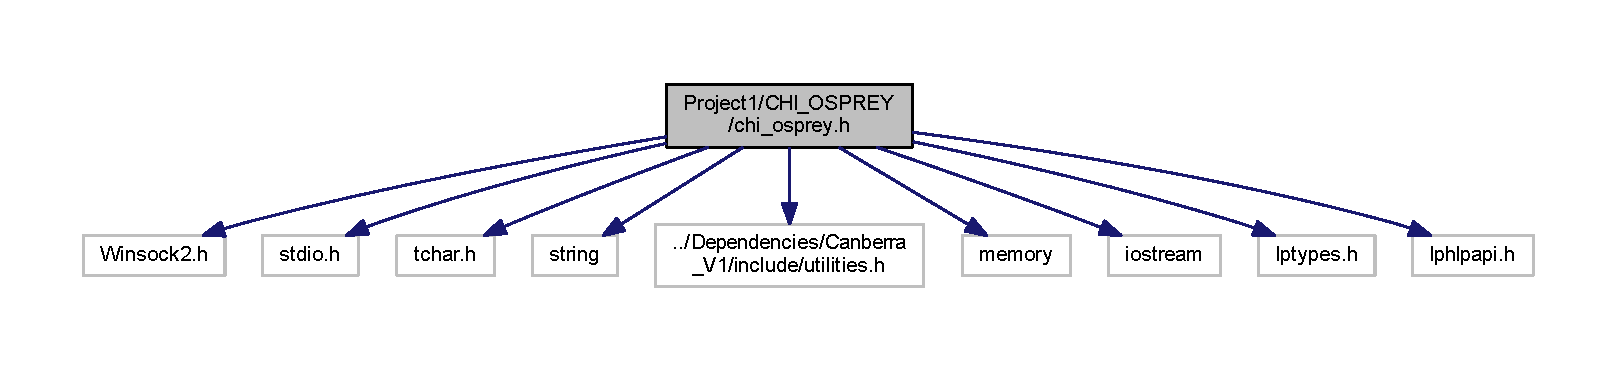
\includegraphics[width=350pt]{d4/d4e/chi__osprey_8h__incl}
\end{center}
\end{figure}
This graph shows which files directly or indirectly include this file\+:\nopagebreak
\begin{figure}[H]
\begin{center}
\leavevmode
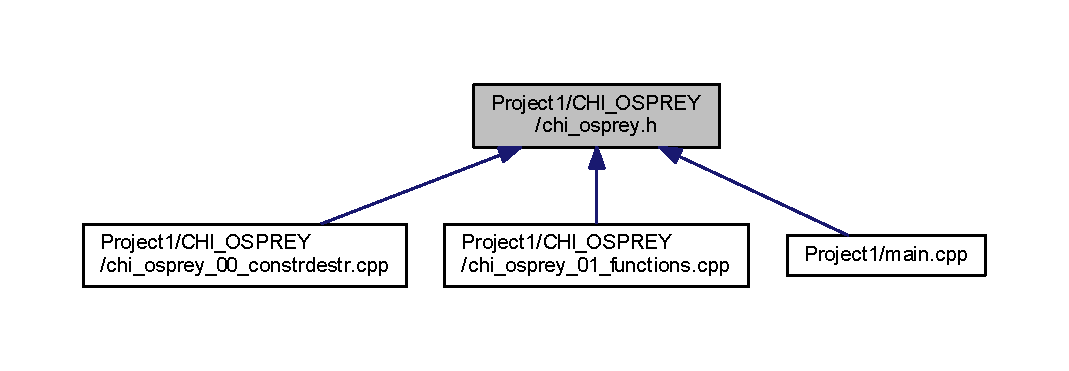
\includegraphics[width=350pt]{df/dc6/chi__osprey_8h__dep__incl}
\end{center}
\end{figure}
\subsection*{Classes}
\begin{DoxyCompactItemize}
\item 
struct \hyperlink{chi__osprey_8h_d2/d7a/struct_c_s_t___o_s_p_r_e_y___i_n_f_o}{C\+S\+T\+\_\+\+O\+S\+P\+R\+E\+Y\+\_\+\+I\+N\+FO}
\item 
class \hyperlink{class_c_h_i___o_s_p_r_e_y}{C\+H\+I\+\_\+\+O\+S\+P\+R\+EY}
\end{DoxyCompactItemize}


\subsection{Class Documentation}
\index{C\+S\+T\+\_\+\+O\+S\+P\+R\+E\+Y\+\_\+\+I\+N\+FO@{C\+S\+T\+\_\+\+O\+S\+P\+R\+E\+Y\+\_\+\+I\+N\+FO}}\label{struct_c_s_t___o_s_p_r_e_y___i_n_f_o}
\Hypertarget{chi__osprey_8h_struct_c_s_t___o_s_p_r_e_y___i_n_f_o}
\subsubsection{struct C\+S\+T\+\_\+\+O\+S\+P\+R\+E\+Y\+\_\+\+I\+N\+FO}


Definition at line 18 of file chi\+\_\+osprey.\+h.

\begin{DoxyFields}{Class Members}
\mbox{\Hypertarget{chi__osprey_8h_a3668cf64637a9d61481f740f39b9e7d8}\label{chi__osprey_8h_a3668cf64637a9d61481f740f39b9e7d8}} 
string&
acquisitionSleepTime&
\\
\hline

\mbox{\Hypertarget{chi__osprey_8h_a84b57c81785927b3f664ca366c674aa4}\label{chi__osprey_8h_a84b57c81785927b3f664ca366c674aa4}} 
string&
calibrationSleepTime&
\\
\hline

\mbox{\Hypertarget{chi__osprey_8h_a15cf8fd34c53039735f2553201d111cd}\label{chi__osprey_8h_a15cf8fd34c53039735f2553201d111cd}} 
string&
channelBounds\mbox{[}10\mbox{]}&
\\
\hline

\mbox{\Hypertarget{chi__osprey_8h_ac22eefe0f719df5a7980dc27559cf7c2}\label{chi__osprey_8h_ac22eefe0f719df5a7980dc27559cf7c2}} 
string&
ipAddress&
\\
\hline

\mbox{\Hypertarget{chi__osprey_8h_a4aeec24f34c07993a2f44ac2f59bd163}\label{chi__osprey_8h_a4aeec24f34c07993a2f44ac2f59bd163}} 
string&
ospreyID&
\\
\hline

\end{DoxyFields}

\hypertarget{chi__osprey__00__constrdestr_8cpp}{}\section{Project1/\+C\+H\+I\+\_\+\+O\+S\+P\+R\+E\+Y/chi\+\_\+osprey\+\_\+00\+\_\+constrdestr.cpp File Reference}
\label{chi__osprey__00__constrdestr_8cpp}\index{Project1/\+C\+H\+I\+\_\+\+O\+S\+P\+R\+E\+Y/chi\+\_\+osprey\+\_\+00\+\_\+constrdestr.\+cpp@{Project1/\+C\+H\+I\+\_\+\+O\+S\+P\+R\+E\+Y/chi\+\_\+osprey\+\_\+00\+\_\+constrdestr.\+cpp}}
{\ttfamily \#include \char`\"{}chi\+\_\+osprey.\+h\char`\"{}}\newline
Include dependency graph for chi\+\_\+osprey\+\_\+00\+\_\+constrdestr.\+cpp\+:\nopagebreak
\begin{figure}[H]
\begin{center}
\leavevmode
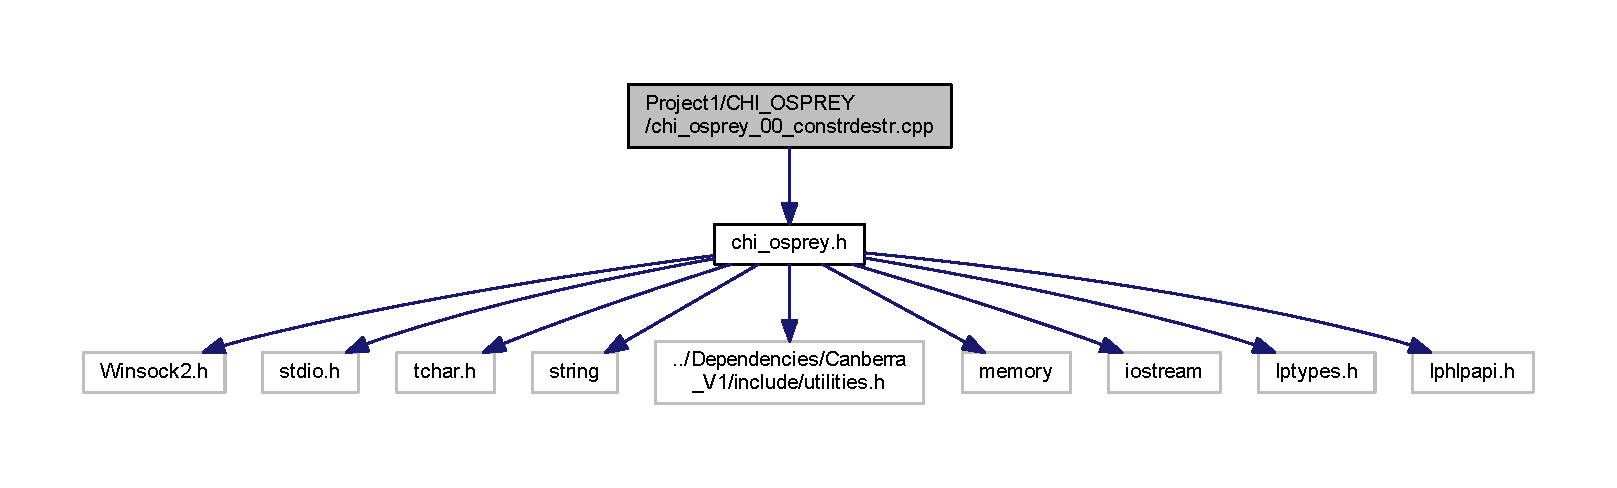
\includegraphics[width=350pt]{d1/dc1/chi__osprey__00__constrdestr_8cpp__incl}
\end{center}
\end{figure}

\hypertarget{chi__osprey__01__functions_8cpp}{}\section{Project1/\+C\+H\+I\+\_\+\+O\+S\+P\+R\+E\+Y/chi\+\_\+osprey\+\_\+01\+\_\+functions.cpp File Reference}
\label{chi__osprey__01__functions_8cpp}\index{Project1/\+C\+H\+I\+\_\+\+O\+S\+P\+R\+E\+Y/chi\+\_\+osprey\+\_\+01\+\_\+functions.\+cpp@{Project1/\+C\+H\+I\+\_\+\+O\+S\+P\+R\+E\+Y/chi\+\_\+osprey\+\_\+01\+\_\+functions.\+cpp}}
{\ttfamily \#include $<$iostream$>$}\newline
{\ttfamily \#include $<$string$>$}\newline
{\ttfamily \#include $<$fstream$>$}\newline
{\ttfamily \#include $<$iterator$>$}\newline
{\ttfamily \#include $<$sstream$>$}\newline
{\ttfamily \#include \char`\"{}../\+Dependencies/\+Canberra\+\_\+\+V1/include/utilities.\+h\char`\"{}}\newline
{\ttfamily \#include \char`\"{}../\+C\+H\+I\+\_\+\+V\+E\+C\+T\+O\+R/chi\+\_\+vector.\+h\char`\"{}}\newline
{\ttfamily \#include \char`\"{}chi\+\_\+osprey.\+h\char`\"{}}\newline
Include dependency graph for chi\+\_\+osprey\+\_\+01\+\_\+functions.\+cpp\+:\nopagebreak
\begin{figure}[H]
\begin{center}
\leavevmode
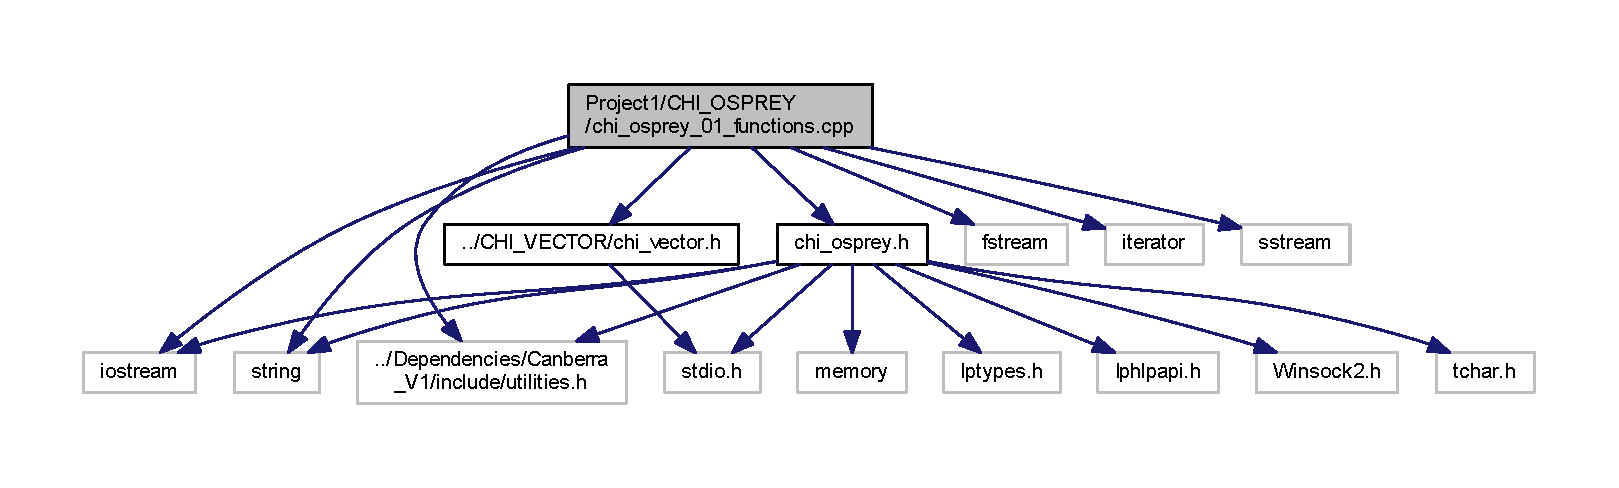
\includegraphics[width=350pt]{dc/dba/chi__osprey__01__functions_8cpp__incl}
\end{center}
\end{figure}
\subsection*{Variables}
\begin{DoxyCompactItemize}
\item 
\mbox{\Hypertarget{chi__osprey__01__functions_8cpp_ab4018c51a1a2cb2d616245c86a1cd61c}\label{chi__osprey__01__functions_8cpp_ab4018c51a1a2cb2d616245c86a1cd61c}} 
\hyperlink{class_c_h_i___v_e_c_t_o_r}{C\+H\+I\+\_\+\+V\+E\+C\+T\+OR}$<$ \hyperlink{class_c_h_i___o_s_p_r_e_y}{C\+H\+I\+\_\+\+O\+S\+P\+R\+EY} $>$ \hyperlink{chi__osprey__01__functions_8cpp_ab4018c51a1a2cb2d616245c86a1cd61c}{osprey\+Stack}
\begin{DoxyCompactList}\small\item\em Osprey Object. \end{DoxyCompactList}\end{DoxyCompactItemize}

\hypertarget{chi__vector_8h}{}\section{Project1/\+C\+H\+I\+\_\+\+V\+E\+C\+T\+O\+R/chi\+\_\+vector.h File Reference}
\label{chi__vector_8h}\index{Project1/\+C\+H\+I\+\_\+\+V\+E\+C\+T\+O\+R/chi\+\_\+vector.\+h@{Project1/\+C\+H\+I\+\_\+\+V\+E\+C\+T\+O\+R/chi\+\_\+vector.\+h}}
{\ttfamily \#include $<$stdio.\+h$>$}\newline
Include dependency graph for chi\+\_\+vector.\+h\+:\nopagebreak
\begin{figure}[H]
\begin{center}
\leavevmode
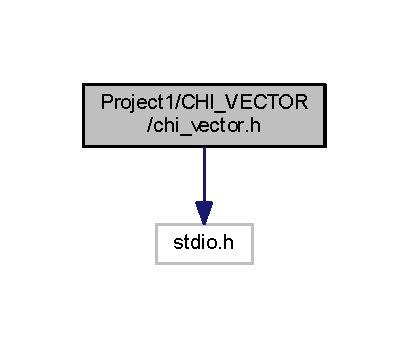
\includegraphics[width=196pt]{d0/d25/chi__vector_8h__incl}
\end{center}
\end{figure}
This graph shows which files directly or indirectly include this file\+:\nopagebreak
\begin{figure}[H]
\begin{center}
\leavevmode
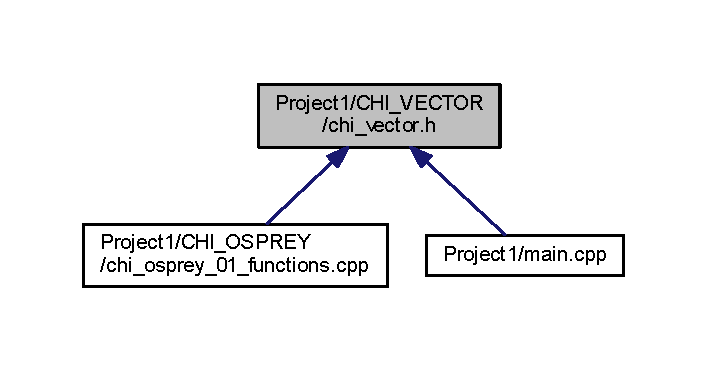
\includegraphics[width=340pt]{db/d30/chi__vector_8h__dep__incl}
\end{center}
\end{figure}
\subsection*{Classes}
\begin{DoxyCompactItemize}
\item 
class \hyperlink{class_c_h_i___v_e_c_t_o_r}{C\+H\+I\+\_\+\+V\+E\+C\+T\+O\+R$<$ Vector\+Type $>$}
\end{DoxyCompactItemize}

\hypertarget{main_8cpp}{}\section{Project1/main.cpp File Reference}
\label{main_8cpp}\index{Project1/main.\+cpp@{Project1/main.\+cpp}}
{\ttfamily \#include $<$iostream$>$}\newline
{\ttfamily \#include $<$fstream$>$}\newline
{\ttfamily \#include $<$signal.\+h$>$}\newline
{\ttfamily \#include $<$math.\+h$>$}\newline
{\ttfamily \#include $<$string$>$}\newline
{\ttfamily \#include $<$time.\+h$>$}\newline
{\ttfamily \#include \char`\"{}C\+H\+I\+\_\+\+O\+S\+P\+R\+E\+Y\textbackslash{}chi\+\_\+osprey.\+h\char`\"{}}\newline
{\ttfamily \#include \char`\"{}C\+H\+I\+\_\+\+V\+E\+C\+T\+O\+R\textbackslash{}chi\+\_\+vector.\+h\char`\"{}}\newline
Include dependency graph for main.\+cpp\+:\nopagebreak
\begin{figure}[H]
\begin{center}
\leavevmode
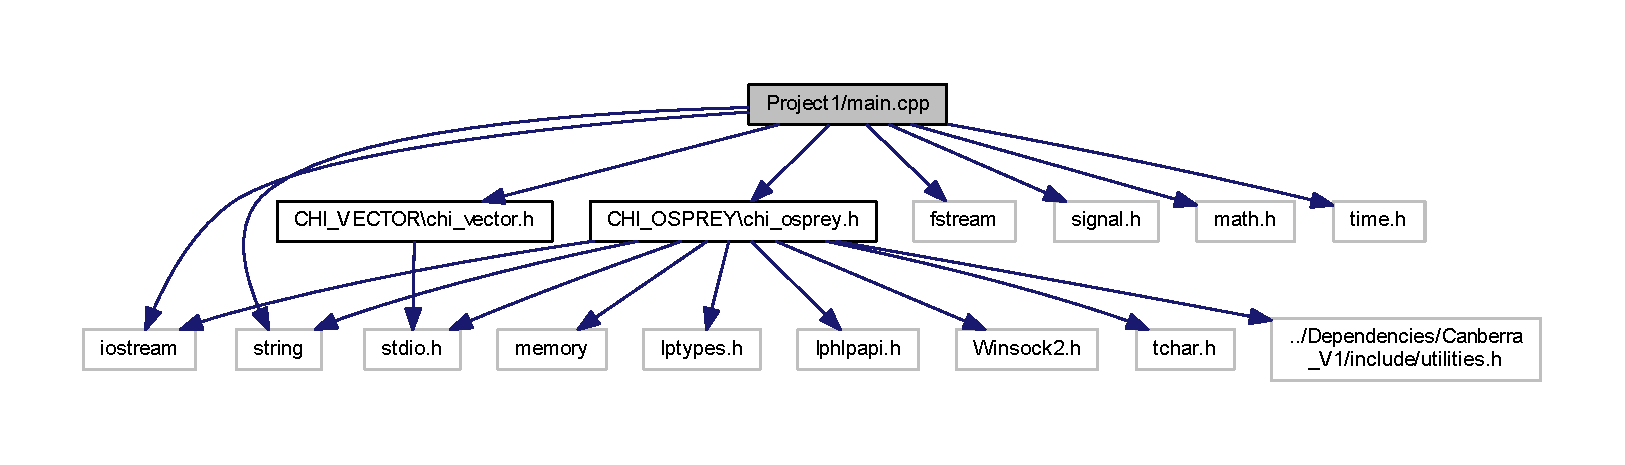
\includegraphics[width=350pt]{da/dce/main_8cpp__incl}
\end{center}
\end{figure}
\subsection*{Classes}
\begin{DoxyCompactItemize}
\item 
struct \hyperlink{main_8cpp_d2/d03/struct_c_s_t___m_a_p_p_i_n_g}{C\+S\+T\+\_\+\+M\+A\+P\+P\+I\+NG}
\end{DoxyCompactItemize}
\subsection*{Macros}
\begin{DoxyCompactItemize}
\item 
\mbox{\Hypertarget{main_8cpp_ac50762666aa00bd3a4308158510f1748}\label{main_8cpp_ac50762666aa00bd3a4308158510f1748}} 
\#define {\bfseries \+\_\+\+W\+I\+N32\+\_\+\+W\+I\+N\+NT}~0x0501
\end{DoxyCompactItemize}
\subsection*{Functions}
\begin{DoxyCompactItemize}
\item 
void \hyperlink{main_8cpp_a00c44aa4276ad8c70f0bd1be93002a66_a00c44aa4276ad8c70f0bd1be93002a66}{Osprey\+Parse\+Input} (std\+::string file\+Name)
\begin{DoxyCompactList}\small\item\em Utility Function used for parsing the input file. \end{DoxyCompactList}\item 
std\+::string \hyperlink{main_8cpp_abecada661ceb15d45a4267ebee66c637_abecada661ceb15d45a4267ebee66c637}{Osprey\+Extract\+String} (std\+::string str, char beg, char end)
\begin{DoxyCompactList}\small\item\em Utility Function used for extracting a substring. \end{DoxyCompactList}\item 
void \hyperlink{main_8cpp_a833a814abde34e116c360fbfd06a6193_a833a814abde34e116c360fbfd06a6193}{Sig\+Break\+\_\+\+Handler} (int n\+\_\+signal)
\begin{DoxyCompactList}\small\item\em Utility Function used for exiting the program. \end{DoxyCompactList}\item 
int \hyperlink{main_8cpp_ae66f6b31b5ad750f1fe042a706a4e3d4_ae66f6b31b5ad750f1fe042a706a4e3d4}{main} ()
\end{DoxyCompactItemize}
\subsection*{Variables}
\begin{DoxyCompactItemize}
\item 
\mbox{\Hypertarget{main_8cpp_a0d2117f1e8077a8a7b7175edaa068d57}\label{main_8cpp_a0d2117f1e8077a8a7b7175edaa068d57}} 
bool \hyperlink{main_8cpp_a0d2117f1e8077a8a7b7175edaa068d57}{loop\+Count} = true
\begin{DoxyCompactList}\small\item\em Checks to see if the program has looped before. \end{DoxyCompactList}\item 
\mbox{\Hypertarget{main_8cpp_a73f7a2c9f70067d4f45ddcb6a7dba5f0}\label{main_8cpp_a73f7a2c9f70067d4f45ddcb6a7dba5f0}} 
bool \hyperlink{main_8cpp_a73f7a2c9f70067d4f45ddcb6a7dba5f0}{close\+Program} = false
\begin{DoxyCompactList}\small\item\em Handle to close the program. \end{DoxyCompactList}\item 
\mbox{\Hypertarget{main_8cpp_a5040252e575ddcc2bbfb251abe90e447}\label{main_8cpp_a5040252e575ddcc2bbfb251abe90e447}} 
bool \hyperlink{main_8cpp_a5040252e575ddcc2bbfb251abe90e447}{calibration\+Mode} = false
\begin{DoxyCompactList}\small\item\em Usermode if it should be in calibration mode or run mode. \end{DoxyCompactList}\item 
\mbox{\Hypertarget{main_8cpp_ab9ec31522d06b675fd50036e752dcc84}\label{main_8cpp_ab9ec31522d06b675fd50036e752dcc84}} 
\hyperlink{class_c_h_i___o_s_p_r_e_y}{C\+H\+I\+\_\+\+O\+S\+P\+R\+EY} \hyperlink{main_8cpp_ab9ec31522d06b675fd50036e752dcc84}{osprey} \mbox{[}5\mbox{]}
\begin{DoxyCompactList}\small\item\em Array of ospreys. \end{DoxyCompactList}\item 
\mbox{\Hypertarget{main_8cpp_ab4018c51a1a2cb2d616245c86a1cd61c}\label{main_8cpp_ab4018c51a1a2cb2d616245c86a1cd61c}} 
\hyperlink{class_c_h_i___v_e_c_t_o_r}{C\+H\+I\+\_\+\+V\+E\+C\+T\+OR}$<$ \hyperlink{class_c_h_i___o_s_p_r_e_y}{C\+H\+I\+\_\+\+O\+S\+P\+R\+EY} $>$ \hyperlink{main_8cpp_ab4018c51a1a2cb2d616245c86a1cd61c}{osprey\+Stack}
\begin{DoxyCompactList}\small\item\em Osprey Object. \end{DoxyCompactList}\end{DoxyCompactItemize}


\subsection{Class Documentation}
\index{C\+S\+T\+\_\+\+M\+A\+P\+P\+I\+NG@{C\+S\+T\+\_\+\+M\+A\+P\+P\+I\+NG}}\label{struct_c_s_t___m_a_p_p_i_n_g}
\Hypertarget{main_8cpp_struct_c_s_t___m_a_p_p_i_n_g}
\subsubsection{struct C\+S\+T\+\_\+\+M\+A\+P\+P\+I\+NG}
Structure initializing information for memory mapping. 

Definition at line 31 of file main.\+cpp.

\begin{DoxyFields}{Class Members}
\mbox{\Hypertarget{main_8cpp_a00b4c49d7f865a80b2b92ef60049ae4c}\label{main_8cpp_a00b4c49d7f865a80b2b92ef60049ae4c}} 
float&
fTime&
Time in seconds. \\
\hline

\mbox{\Hypertarget{main_8cpp_a15a94aba68ce13addacd8a8541fee0e5}\label{main_8cpp_a15a94aba68ce13addacd8a8541fee0e5}} 
float&
ospreyChannels\mbox{[}25\mbox{]}&
Total channels for 5 ospreys. \\
\hline

\end{DoxyFields}


\subsection{Function Documentation}
\mbox{\Hypertarget{main_8cpp_ae66f6b31b5ad750f1fe042a706a4e3d4_ae66f6b31b5ad750f1fe042a706a4e3d4}\label{main_8cpp_ae66f6b31b5ad750f1fe042a706a4e3d4_ae66f6b31b5ad750f1fe042a706a4e3d4}} 
\index{main.\+cpp@{main.\+cpp}!main@{main}}
\index{main@{main}!main.\+cpp@{main.\+cpp}}
\subsubsection{\texorpdfstring{main()}{main()}}
{\footnotesize\ttfamily int main (\begin{DoxyParamCaption}{ }\end{DoxyParamCaption})}

Main function \begin{DoxyAuthor}{Author}
Guillermo Villanueva 
\end{DoxyAuthor}


Definition at line 55 of file main.\+cpp.


\begin{DoxyCode}
56 \{
57     \textcolor{comment}{//===================================================== Intializing Past Date for Timing}
58     time\_t sTimer;
59     \textcolor{keyword}{struct }tm pastTime = \{ 0 \};
60     \textcolor{keywordtype}{double} tSeconds;
61     pastTime.tm\_year = 100;
62     pastTime.tm\_mon = 0;
63     pastTime.tm\_mday = 1;
64     pastTime.tm\_hour = 0;
65     pastTime.tm\_min = 0;
66     pastTime.tm\_sec = 0;
67 
68     \textcolor{comment}{//===================================================== Introductory text}
69     printf(\textcolor{stringliteral}{"FAM Channels Mapping Program \(\backslash\)n"});
70 
71     \textcolor{comment}{//===================================================== Get a handle for a file mapping}
72     HANDLE fileHandle=CreateFileMapping(    INVALID\_HANDLE\_VALUE,
73                                             NULL,                    \textcolor{comment}{// default security}
74                                             PAGE\_READWRITE,          \textcolor{comment}{// read/write access}
75                                             0,                       \textcolor{comment}{// maximum object size (high-order
       DWORD)}
76                                             8,                       \textcolor{comment}{// maximum object size (low-order
       DWORD)}
77                                             \textcolor{stringliteral}{"FAM\_CHANNELS"});        \textcolor{comment}{// name of mapping object)}
78 
79     \textcolor{comment}{//===================================================== Handle error}
80     \textcolor{keywordflow}{if} (fileHandle==NULL)
81     \{
82         std::cout << \textcolor{stringliteral}{"ERROR: Could not create file mapping\(\backslash\)n"};
83         \textcolor{keywordflow}{return} 0;
84     \}
85     
86     \textcolor{comment}{//===================================================== Creating a new map to copy over.}
87     \hyperlink{main_8cpp_d2/d03/struct_c_s_t___m_a_p_p_i_n_g}{CST\_MAPPING}* newMap = (\hyperlink{main_8cpp_d2/d03/struct_c_s_t___m_a_p_p_i_n_g}{CST\_MAPPING}*)MapViewOfFile(        fileHandle,            
       \textcolor{comment}{// handle to map object}
88                                              FILE\_MAP\_ALL\_ACCESS,   \textcolor{comment}{// read/write permission}
89                                              0,
90                                              0,
91                                              \textcolor{keyword}{sizeof}(\hyperlink{main_8cpp_d2/d03/struct_c_s_t___m_a_p_p_i_n_g}{CST\_MAPPING}));
92 
93     \textcolor{comment}{//===================================================== Handle error}
94     \textcolor{keywordflow}{if} (newMap==NULL)
95     \{
96         std::cout << \textcolor{stringliteral}{"ERROR: Could not map view of file\(\backslash\)n"};
97         \textcolor{keywordflow}{return} 0;
98     \}
99 
100     \textcolor{comment}{//===================================================== Copy over initial variables}
101     \hyperlink{main_8cpp_d2/d03/struct_c_s_t___m_a_p_p_i_n_g}{CST\_MAPPING} intValues;
102     intValues.\hyperlink{main_8cpp_a00b4c49d7f865a80b2b92ef60049ae4c}{fTime} = 0;
103     \textcolor{keywordflow}{for} (\textcolor{keywordtype}{int} i = 0; i < 25; i++)
104     \{
105         intValues.\hyperlink{main_8cpp_a15a94aba68ce13addacd8a8541fee0e5}{ospreyChannels}[i] = 0;
106     \}
107 
108     CopyMemory(newMap, &intValues, \textcolor{keyword}{sizeof}(\hyperlink{main_8cpp_d2/d03/struct_c_s_t___m_a_p_p_i_n_g}{CST\_MAPPING}));
109 
110 
111     \textcolor{comment}{//===================================================== Create a windows waitable timer (minimizes CPU
       usage)}
112     HANDLE hTimer = CreateWaitableTimer(NULL,                   \textcolor{comment}{// Default security attributes}
113                                         NULL,                  \textcolor{comment}{// Create auto-reset timer}
114                                         TEXT(\textcolor{stringliteral}{"FAMTIMER"}));       \textcolor{comment}{// Name of waitable timer}
115 
116     \textcolor{comment}{//===================================================== Set timer parameters}
117     \_\_int64         qwDueTime;
118     LARGE\_INTEGER   liDueTime;
119     qwDueTime = -0 * 10000000;
120     liDueTime.LowPart  = (DWORD) ( qwDueTime & 0xFFFFFFFF );
121     liDueTime.HighPart = (LONG)  ( qwDueTime >> 32 );
122 
123     BOOL bSuccess = SetWaitableTimer(
124                 hTimer,           \textcolor{comment}{// Handle to the timer object}
125                 &liDueTime,       \textcolor{comment}{// When timer will become signaled}
126                 16,             \textcolor{comment}{// Periodic timer interval of 16 milli-seconds}
127                 NULL,     \textcolor{comment}{// Completion routine}
128                 NULL,          \textcolor{comment}{// Argument to the completion routine}
129                 FALSE );          \textcolor{comment}{// Do not restore a suspended system}
130 
131     \textcolor{comment}{//===================================================== Assign close signal handler}
132     signal(SIGBREAK, &\hyperlink{main_8cpp_a833a814abde34e116c360fbfd06a6193_a833a814abde34e116c360fbfd06a6193}{SigBreak\_Handler});
133 
134 
135     \textcolor{comment}{//===================================================== Running Script}
136     \textcolor{keywordtype}{int} acquisitionTime = 500;
137     \textcolor{keywordtype}{int} ospreyCount = \hyperlink{main_8cpp_ab4018c51a1a2cb2d616245c86a1cd61c}{ospreyStack}.itemCount;
138 
139     \hyperlink{main_8cpp_a00c44aa4276ad8c70f0bd1be93002a66_a00c44aa4276ad8c70f0bd1be93002a66}{OspreyParseInput}(\textcolor{stringliteral}{"init.ini"});
140     
141     \textcolor{keywordflow}{for}(\textcolor{keywordtype}{int} k = 0; k < ospreyCount; k++)
142     \{
143         \hyperlink{main_8cpp_ab9ec31522d06b675fd50036e752dcc84}{osprey}[k].OspreyInitialize(k, \hyperlink{main_8cpp_a5040252e575ddcc2bbfb251abe90e447}{calibrationMode});
144     \}
145 
146     time(&sTimer);
147     \textcolor{keywordflow}{while} (\hyperlink{main_8cpp_a0d2117f1e8077a8a7b7175edaa068d57}{loopCount})
148     \{
149         \textcolor{keywordflow}{for} (\textcolor{keywordtype}{int} k = 0; k < ospreyCount; k++)
150         \{
151             \hyperlink{class_c_h_i___o_s_p_r_e_y}{CHI\_OSPREY}* currentOsprey = \hyperlink{main_8cpp_ab4018c51a1a2cb2d616245c86a1cd61c}{ospreyStack}.GetItem(k);
152             \hyperlink{main_8cpp_ab9ec31522d06b675fd50036e752dcc84}{osprey}[k].OspreyPullSpectrums(k, std::stoi(currentOsprey->curOsprey->acquisitionSleepTime
      ));
153             
154             \textcolor{keywordflow}{for} (\textcolor{keywordtype}{int} i = 0; i < 5; i++)
155             \{
156                 intValues.\hyperlink{main_8cpp_a15a94aba68ce13addacd8a8541fee0e5}{ospreyChannels}[5 * k + i] = \hyperlink{main_8cpp_ab9ec31522d06b675fd50036e752dcc84}{osprey}[k].channel[i+1];
157             \}
158         
159         \}
160 
161         intValues.\hyperlink{main_8cpp_a00b4c49d7f865a80b2b92ef60049ae4c}{fTime} = difftime(sTimer, mktime(&pastTime));
162         CopyMemory(newMap, &intValues, \textcolor{keyword}{sizeof}(\hyperlink{main_8cpp_d2/d03/struct_c_s_t___m_a_p_p_i_n_g}{CST\_MAPPING}));
163 
164         \textcolor{keywordflow}{if} (HIBYTE(GetAsyncKeyState(VK\_RETURN))) 
165         \{
166             \hyperlink{main_8cpp_a0d2117f1e8077a8a7b7175edaa068d57}{loopCount} = \textcolor{keyword}{false};
167         \}
168     \}
169 
170     \textcolor{comment}{//===================================================== Close the file handle}
171     UnmapViewOfFile(newMap);
172     CloseHandle(fileHandle);
173 
174     std::cout<<\textcolor{stringliteral}{"Program finished!\(\backslash\)n"};
175 
176     \textcolor{keywordflow}{return} 0;
177 \}
\end{DoxyCode}
\mbox{\Hypertarget{main_8cpp_abecada661ceb15d45a4267ebee66c637_abecada661ceb15d45a4267ebee66c637}\label{main_8cpp_abecada661ceb15d45a4267ebee66c637_abecada661ceb15d45a4267ebee66c637}} 
\index{main.\+cpp@{main.\+cpp}!Osprey\+Extract\+String@{Osprey\+Extract\+String}}
\index{Osprey\+Extract\+String@{Osprey\+Extract\+String}!main.\+cpp@{main.\+cpp}}
\subsubsection{\texorpdfstring{Osprey\+Extract\+String()}{OspreyExtractString()}}
{\footnotesize\ttfamily std\+::string Osprey\+Extract\+String (\begin{DoxyParamCaption}\item[{std\+::string}]{str,  }\item[{char}]{beg,  }\item[{char}]{end }\end{DoxyParamCaption})}



Utility Function used for extracting a substring. 

The function extracts a substring from a given string, that is between two delimiters.


\begin{DoxyParams}{Parameters}
{\em str} & The main string. \\
\hline
{\em beg} & The beginning delimiter. \\
\hline
{\em end} & The ending delimiter.\\
\hline
\end{DoxyParams}
\begin{DoxyAuthor}{Author}
Guillermo Vilanueva 
\end{DoxyAuthor}


Definition at line 193 of file main.\+cpp.


\begin{DoxyCode}
194 \{
195     std::size\_t begPos;
196     \textcolor{keywordflow}{if} ((begPos = str.find(beg)) != std::string::npos)
197     \{
198         std::size\_t endPos;
199         \textcolor{keywordflow}{if} ((endPos = str.find(end, begPos)) != std::string::npos && endPos != begPos + 1)
200             \textcolor{keywordflow}{return} str.substr(begPos + 1, endPos - begPos - 1);
201     \}
202 
203     \textcolor{keywordflow}{return} std::string();
204 \}
\end{DoxyCode}
\mbox{\Hypertarget{main_8cpp_a00c44aa4276ad8c70f0bd1be93002a66_a00c44aa4276ad8c70f0bd1be93002a66}\label{main_8cpp_a00c44aa4276ad8c70f0bd1be93002a66_a00c44aa4276ad8c70f0bd1be93002a66}} 
\index{main.\+cpp@{main.\+cpp}!Osprey\+Parse\+Input@{Osprey\+Parse\+Input}}
\index{Osprey\+Parse\+Input@{Osprey\+Parse\+Input}!main.\+cpp@{main.\+cpp}}
\subsubsection{\texorpdfstring{Osprey\+Parse\+Input()}{OspreyParseInput()}}
{\footnotesize\ttfamily void Osprey\+Parse\+Input (\begin{DoxyParamCaption}\item[{std\+::string}]{file\+Name }\end{DoxyParamCaption})}



Utility Function used for parsing the input file. 

The function extracts the information provided by the input file, and stores the found information into a structure.


\begin{DoxyParams}{Parameters}
{\em file\+Name} & The file to be parsed.\\
\hline
\end{DoxyParams}
\begin{DoxyAuthor}{Author}
Guillermo Vilanueva 
\end{DoxyAuthor}


Definition at line 218 of file main.\+cpp.


\begin{DoxyCode}
219 \{
220     \textcolor{comment}{//==================================== Defining pointer array}
221     \hyperlink{chi__osprey_8h_d2/d7a/struct_c_s_t___o_s_p_r_e_y___i_n_f_o}{CST\_OSPREY\_INFO}* newOsprey;
222     std::string parserStruct[14];
223 
224 
225     \textcolor{comment}{//==================================== Declaring variables}
226     \textcolor{keywordtype}{int} indexCount = 0;
227     \textcolor{keywordtype}{int} ospreyCount = 0;
228     std::string currentLine;
229 
230     \textcolor{comment}{//==================================== Declaring filestream & opening file}
231     std::ifstream inputFile;
232     inputFile.open(fileName);
233 
234     \textcolor{comment}{//==================================== Checking to see if input failed}
235     \textcolor{keywordflow}{if} (!inputFile.is\_open())
236     \{
237         printf(\textcolor{stringliteral}{"File: %s failed to load. \(\backslash\)n"}, fileName.c\_str());
238         \textcolor{keywordflow}{return};
239     \}
240     \textcolor{keywordflow}{else}
241     \{
242         printf(\textcolor{stringliteral}{"File: %s succeeded to load. \(\backslash\)n"}, fileName.c\_str());
243     \}
244 
245     \textcolor{comment}{//==================================== Searchs through loaded file.}
246     \textcolor{keywordflow}{while} (std::getline(inputFile, currentLine))
247     \{
248         \textcolor{comment}{//==================================== Declaring variables}
249         \textcolor{keywordtype}{size\_t} decCount;
250         \textcolor{keywordtype}{size\_t} comCount;        
251         \textcolor{keywordtype}{size\_t} tCount;          
252 
253         std::string mainString;
254         std::string subStringOne;
255         std::string subStringTwo;
256         std::string subStringThree;
257 
258         \textcolor{comment}{//==================================== Parsing lines}
259         mainString = \hyperlink{main_8cpp_abecada661ceb15d45a4267ebee66c637_abecada661ceb15d45a4267ebee66c637}{OspreyExtractString}(currentLine, \textcolor{charliteral}{'('}, \textcolor{charliteral}{')'});
260         subStringOne = mainString.substr(0, mainString.find(\textcolor{charliteral}{','}));
261         subStringTwo = mainString.substr(mainString.find(\textcolor{charliteral}{','}) + 1);
262         subStringThree = mainString.substr(0, mainString.find(\textcolor{charliteral}{'t'}));
263 
264         \textcolor{comment}{//==================================== Counting Occurences}
265         decCount = std::count(mainString.begin(), mainString.end(), \textcolor{charliteral}{'.'});
266         comCount = std::count(mainString.begin(), mainString.end(), \textcolor{charliteral}{','});
267         tCount = std::count(mainString.begin(), mainString.end(), \textcolor{charliteral}{'t'});
268 
269         \textcolor{comment}{//==================================== Checking for delimiter}
270         \textcolor{keywordflow}{if} (currentLine.find(\textcolor{charliteral}{'\{'}) != std::string::npos)
271         \{
272             newOsprey = \textcolor{keyword}{new} \hyperlink{chi__osprey_8h_d2/d7a/struct_c_s_t___o_s_p_r_e_y___i_n_f_o}{CST\_OSPREY\_INFO};
273             ospreyCount = ospreyCount + 1;
274             parserStruct[indexCount] = std::to\_string(ospreyCount);
275             indexCount = indexCount + 1;
276         \}
277 
278         \textcolor{comment}{//==================================== Checking for delimiter}
279         \textcolor{keywordflow}{if} (decCount >= 3)
280         \{
281             parserStruct[indexCount] = mainString;
282             indexCount = indexCount + 1;
283         \}
284 
285         \textcolor{comment}{//==================================== Checking for delimiter}
286         \textcolor{keywordflow}{if} (comCount >= 1)
287         \{
288             parserStruct[indexCount] = subStringOne;
289             indexCount = indexCount + 1;
290             parserStruct[indexCount] = subStringTwo;
291             indexCount = indexCount + 1;
292         \}
293 
294         \textcolor{comment}{//==================================== Checking for delimiter}
295         \textcolor{keywordflow}{if} (tCount >= 1)
296         \{
297             parserStruct[indexCount] = subStringThree;
298             indexCount = indexCount + 1;
299         \}
300 
301 
302 
303         \textcolor{comment}{//==================================== Checking for delimiter & pushing to stack}
304         \textcolor{keywordflow}{if} (currentLine.find(\textcolor{charliteral}{'\}'}) != std::string::npos)
305         \{
306             newOsprey->ospreyID = parserStruct[0];
307             newOsprey->ipAddress = parserStruct[1];
308             \textcolor{keywordflow}{for} (\textcolor{keywordtype}{int} k = 0; k < 10; k++)
309             \{
310                 newOsprey->channelBounds[k] = parserStruct[k+2];
311             \}
312             newOsprey->calibrationSleepTime = parserStruct[12];
313             newOsprey->acquisitionSleepTime = parserStruct[13];
314 
315             \hyperlink{class_c_h_i___o_s_p_r_e_y}{CHI\_OSPREY}* newOspreyObject = \textcolor{keyword}{new} \hyperlink{class_c_h_i___o_s_p_r_e_y}{CHI\_OSPREY};
316             newOspreyObject->curOsprey = newOsprey;
317             \hyperlink{main_8cpp_ab4018c51a1a2cb2d616245c86a1cd61c}{ospreyStack}.PushItem(newOspreyObject);
318 
319 
320             indexCount = 0;
321         \}
322     \}
323 
324     \textcolor{comment}{//==================================== Closing file}
325     inputFile.close();
326     \textcolor{keywordflow}{return};
327 \}
\end{DoxyCode}
\mbox{\Hypertarget{main_8cpp_a833a814abde34e116c360fbfd06a6193_a833a814abde34e116c360fbfd06a6193}\label{main_8cpp_a833a814abde34e116c360fbfd06a6193_a833a814abde34e116c360fbfd06a6193}} 
\index{main.\+cpp@{main.\+cpp}!Sig\+Break\+\_\+\+Handler@{Sig\+Break\+\_\+\+Handler}}
\index{Sig\+Break\+\_\+\+Handler@{Sig\+Break\+\_\+\+Handler}!main.\+cpp@{main.\+cpp}}
\subsubsection{\texorpdfstring{Sig\+Break\+\_\+\+Handler()}{SigBreak\_Handler()}}
{\footnotesize\ttfamily void Sig\+Break\+\_\+\+Handler (\begin{DoxyParamCaption}\item[{int}]{n\+\_\+signal }\end{DoxyParamCaption})}



Utility Function used for exiting the program. 

A signal is passed which calls for the program to be closed.


\begin{DoxyParams}{Parameters}
{\em n\+\_\+signal} & The signal to be passed.\\
\hline
\end{DoxyParams}
\begin{DoxyAuthor}{Author}
Guillermo Vilanueva 
\end{DoxyAuthor}


Definition at line 340 of file main.\+cpp.


\begin{DoxyCode}
341 \{
342     \hyperlink{main_8cpp_a73f7a2c9f70067d4f45ddcb6a7dba5f0}{closeProgram} = \textcolor{keyword}{true};
343 \}
\end{DoxyCode}

%--- End generated contents ---

% Index
\backmatter
\newpage
\phantomsection
\clearemptydoublepage
\addcontentsline{toc}{chapter}{Index}
\printindex

\end{document}
